%% 说明:请用 PdfLatex 编译!
\documentclass[a4paper]{article}
\usepackage[text={170mm, 245mm}, centering]{geometry} %页面设置
\usepackage[UTF8]{ctex}
\usepackage{amsmath, amsthm, amssymb} %数学公式、数学符号
\usepackage{xcolor}
\usepackage{graphicx} % 插图
\usepackage{epstopdf} 
\usepackage{fancyhdr} % 页眉页脚设置
\usepackage{enumerate, enumitem}%项目列表 
\usepackage{booktabs}
\usepackage{multirow} %多行
\usepackage{array}
\usepackage{tabularx}
\usepackage{setspace}%行间距
\usepackage[pdftex, colorlinks, linkcolor=blue, anchorcolor=blue, citecolor=blue]{hyperref} %超链接
\usepackage{graphicx}
\usepackage{algorithm, algorithmicx, algpseudocode}   
% \usepackage[capitalise, noabbrev]{cleveref} %自动识别引用对象的类型, 并打印出对应的引用p
\usepackage[square,  comma,  sort&compress, numbers]{natbib}
% \renewcommand\citep[1]{[\citeauthor{#1},  \citeyear{#1}]}
\newcommand{\SUB}[1]{\ENSURE \hspace{-0.15in} \textbf{#1}}
\newcommand{\FOR}{ \State \textbf{for }}
\newcommand{\lbs}{\ensuremath{B}}     
\newcommand{\lepochs}{\ensuremath{E}}
\newcommand{\mycaptionof}[2]{\captionof{#1}{#2}}

\usepackage{tikz-cd}
\usepackage{url}
\usepackage{pythonhighlight}  % python code

\graphicspath{{figures/}} %设定存放图片的路径
\bibliographystyle{plainnat} %参考文献格式定义

\setlength{\headheight}{14pt} 
%%=====页眉页脚设置=========================================
\pagestyle{fancy}
\lhead{\small \it 更新于:\today}
\chead{\small \emph{学习笔记}}
\rhead{\small \thepage}
\lfoot{}
\cfoot{}
\rfoot{}
\renewcommand\headrulewidth{0.5pt} % Size of the header rule

%%=======================================================



%%===================item列表行距======================= 
\setenumerate[1]{leftmargin=1.5em, labelsep=0.5em, itemindent=1em, itemsep=0pt, partopsep=0pt, parsep=\parskip, topsep=0pt}
\setitemize[1]{itemindent=1em, itemsep=0pt, partopsep=0pt, parsep=\parskip, topsep=0pt}
\setdescription[1]{itemindent=0.5em, itemsep=0pt, partopsep=0pt, parsep=\parskip, topsep=0pt} 
\setitemize[2]{itemsep=0pt, partopsep=0pt, parsep=\parskip, topsep=0pt}
%%===================================================

%%=======自定义命令======================================
%% 请把自定义的命令放在这一部分中==========================
\newcommand{\tabincell}[2]{\begin{tabular}{@{}#1@{}}#2\end{tabular}}  
     

\floatname{algorithm}{算法}  
\renewcommand{\algorithmicrequire}{\textbf{输入:}}  
\renewcommand{\algorithmicensure}{\textbf{输出:}}  
\newcommand{\parinterval}{\noindent\hspace{2em}}%定义变量替代原来开头的控制缩进
\DeclareMathOperator*{\argmax}{arg\, max}
\DeclareMathOperator*{\argmin}{arg\, min}
% Use smallcaps (\textsc) or \texttt for algorithms?
% \newcommand{\algfont}[1]{\texttt{#1}}
% \renewcommand{\algorithmicensure}{}
%%======================================================

\title{联邦学习算法研究}
\author{孙博}
\date{\today}


\begin{document}
%%========论文标题===========================

\maketitle
%生成文档目录
\tableofcontents 

\newpage
\centerline{\huge \bf 联邦学习算法研究}
\vspace{5mm}
\centerline{%
孙博\footnote{孙博, 2019级硕士研究生, 苏州蒙纳士联合研究生学院, 邮箱:ericsun20@qq.com.} 
}
\vspace{5mm}
%%========以下为论文正文=====================

\section*{摘要}

% 你利用该模板总结自己学习的知识、阅读的论文以及自己的想法.关于理论知识, 重点是矩阵论、优化理论.

% 你先精读文献 \citep{arxiv-Kairouz-Mcmahan-etc2019}, 
本文为文献 Advances and Open Problems in Federated Learning \citep{arxiv-Kairouz-Mcmahan-etc2019} 的笔记, 该文献介绍了联邦学习的最新进展, 相关研究方向.
  
联邦学习是一种机器学习架构, 在中央服务器或服务提供商的协调下, 多个实体(客户机)协作解决机器学习问题.每个客户的原始数据存储在本地, 不进行交换或传输;相反, 用于即时聚合的重点更新用于实现学习目标. 

在这种设置中, 许多客户(例如移动设备或整个组织)在中央服务器(例如服务提供商)的协调下协作地训练模型, 同时保持训练数据分散.FL体现了集中数据收集和最小化的原则, 可以减轻由于传统的、集中的机器学习和数据科学方法所带来的许多系统隐私风险和成本.在FL研究爆炸性增长的推动下, 本文讨论了近年来的进展, 并提出了大量的开放问题和挑战. 

规范的联邦学习问题涉及到从存储在数以万计的远程设备上的数据学习单个全局统计模型.我们的目标是在这样的约束下学习这个模型, 设备生成的数据在本地存储和处理, 只有中间更新与中央服务器定期通信.目标可以用下列目标函数表示:
\begin{align*}
    \min_w \,  F(w) \,  ,  \, \, \,  \text{其中} \, \, \,  F(w) := \sum_{k=1}^m p_k F_k(w) \,  . \label{eq:original_obj}
\end{align*}
这里 $m$ 为设备总数,  $p_k \geq 0$ and $\sum_k p_k=1$,   $F_k$是设备$k$的局部目标函数.局部目标函数通常定义为局部数据的经验风险,  即 $F_k(w) = \frac{1}{n_k}\sum_{j_k=1}^{n_k} f_{j_k}(w; x_{j_k},  y_{j_k})$,  其中$n_k$是本地可用的样本数量. 用户定义的术语 $p_k$指定每个设备的相对影响, 两个原始设置分别是$p_k=\frac{1}{n}$或$p_k=\frac{n_k}{n}$, 其中$n=\sum_k n_k$是样本的总数.\citep{li2019federated}
 

\section{背景介绍}

\emph{机器学习的基本框架是什么?数据、模型、训练(优化)、预测?}

机器学习方法三个基本要素:模型、学习准则、优化算法.

在实际任务中使用机器学习模型一般会包含以下几个
步骤(如图1.2所示):
数据预处理:经过数据的预处理, 如去除噪声等. 比如在文本分类中, 去除停用词等.
(2) 特征提取:从原始数据中提取一些有效的特征. 比如在图像分类中, 提取边缘、尺度不变特征变换(Scale Invariant Feature Transform, SIFT)特征等.
(3) 特征转换:对特征进行一定的加工, 比如降维和升维. 很多特征转换方法也都是机器学习方法.
降维包括特征抽取(Feature Extraction)和特征选择(Feature Selection)两种途径. 常用的特征转换方法有主成分分析(Principal Components Analysis, PCA)、线性判别分析(Linear Discriminant Analysis, LDA)等.
(4) 预测:机器学习的核心部分, 学习一个函数并进行预测.



% 你在读该论文时自己也要做好资料搜集工作, 整理联邦学习算法的相关背景(包括为什么要研究联邦学习算法).在这之前, 你需要了解机器学习的基本原理.

\emph{为什么要研究联邦学习?最初提出该概念的目的是什么?结合具体的实例进行说明:隐私性需求、跨数据集、跨平台协作学习}

2016年AlphaGo击败了顶尖的人类围棋玩家,  人类希望人工智能(AI)可以更多的领域发挥作用. 
但是现实情况中会遇到相当多问题:   
\begin{enumerate}
    \item 隐私性需求:在当今对隐私要求越来越严格的情况下, 如果外部机构使用医院患者, 银行客户的数据, 必须保证数据不泄露; 保险公司渴望应用非保险行业数据提升解决方案能力.
    \item 跨数据集: 在人工智能驱动的产品推荐服务中, 产品销售商拥有产品信息、用户购买数据, 但没有描述用户购买能力和支付习惯的数据.在大多数行业中, 数据以孤岛的形式存在.由于行业竞争、隐私安全和复杂的管理程序, 甚至同一公司不同部门之间的数据集成也面临着巨大的阻力.几乎不可能将分散在全国各地的数据和机构进行整合, 否则成本是难以承受的.
    \item 跨平台: 数据是分散的, 每家应用的数据不一样,  如社交属性数据、电商交易数据、信用数据,  如何进行跨组织间的数据合作, 会有很大的挑战

    
\end{enumerate} 
 
 
针对以上问题, 研究人员对此的解决方案有:
\citep{yang2019federated}
\begin{enumerate}    
\item 2016年谷歌提出联邦学习 (the federated learning framework).
\citep{brendan2016communication}
\item 杨强团队提出一个全面的、安全的联邦学习框架(a comprehensive secure federated learning framework)(包括:横向联邦学习、纵向联邦学习、迁移联邦学习).
%%\emph{这三类学习机制之间的区别是什么?各有什么应用场景?}
\item 建议在基于联邦机制的组织之间建立数据网络, 这是一种有效的解决方案, 可以在不损害用户隐私的情况下共享知识.  
\end{enumerate} 

\section{研究现状} 
联邦学习这一术语由 McMahan 等人在 2016 年首次提出, 但是在这一术语诞生之前, 已经就存在了大量相关研究工作致力于数据隐私保护, 例如20世纪80年代就已出现的计算加密数据的加密方法.

联邦学习最初只是强调移动和边缘设备应用, 研究者并把这两种设置分别称作跨设备(cross-device)和 跨孤井(cross-silo).基于这两种变体, 这篇论文给联邦学习下了一个更加广泛的定义:联邦学习是多个实体(客户端)协作解决机器学习问题的机器学习设置, 它在一个中央服务器或服务提供商的协调下进行.每个客户端的原始数据存储在本地, 无法交换或迁移, 联邦学习利用局部更新(用于立即聚合 (immediate aggregation))来实现学习目标.
%%研究进展, 发展脉络

\subsection{相关概念}

\subsubsection{定义}

 
定义$N$数据所有者 $\{\mathcal{F}_1, ...\mathcal{F}_N\}$, 它们都希望通过合并各自的数据$\{\mathcal{D}_1, ...\mathcal{D}_N\}$来训练机器学习模型.
传统的方法是将所有数据放在一起, 使用$\mathcal{D} = \mathcal{D}_1 \cup ...\cup\mathcal{D}_N$ 来训练一个模型 $\mathcal{M}_{SUM}$.
联合学习系统是一个学习的过程, 数据所有者合作训练模型$\mathcal {M} _{美联储}$, 在处理任何数据所有者$ \mathcal {F} _i$不公开其数据$\mathcal {D} _i$  \footnote{数据安全的定义在不同的场景中可能有所不同, 但需要提供意义的隐私保证.我们将在第2.3节中演示安全定义的示例.}
另外, $\mathcal{M}_{FED}$, 即$\mathcal{V}_{FED}$的精度应该非常接近$\mathcal{M}_{SUM}$、$\mathcal{V}_{SUM}$的性能.
形式上, 让$\delta$是一个非负实数, 如果
\begin{equation}\label{define}
 \mid \mathcal{V}_{FED} - \mathcal{V}_{SUM} \mid < \delta
\end{equation}


\subsubsection{联邦学习的分类} 
根据数据集分布情况, 可以将联邦学习分为以下三个类别:横向联邦学习、纵向联邦学习与联邦迁移学习.
\begin{figure}
    \centering
    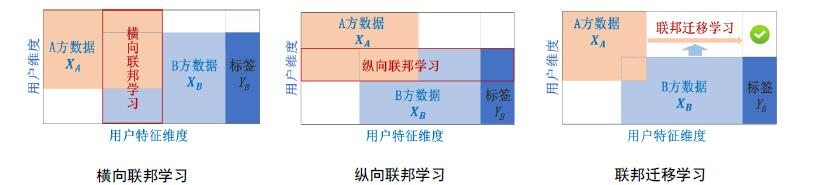
\includegraphics[width=\textwidth]{Categorization_of_FL.jpg}
    \caption{联邦学习的类别}
\end{figure}
\paragraph{横向联邦学习}  横向联邦学习的本质是样本的联合, 适用于参与者间业态相同但客户不同, 即特征重叠多, 用户重叠少时的场景, 比如不同地区的银行间, 他们的业务相似(特征相似), 但用户不同(样本不同).比如有两家不同地区银行, 它们的用户群体分别来自各自所在的地区, 相互的交集很小.但是, 它们的业务很相似, 因此, 记录的用户特征是相同的.此时,  就可以使用横向联邦学习来构建联合模型. 
 
\begin{figure}
    \centering
    \label{Architecture for horizontal FL}
    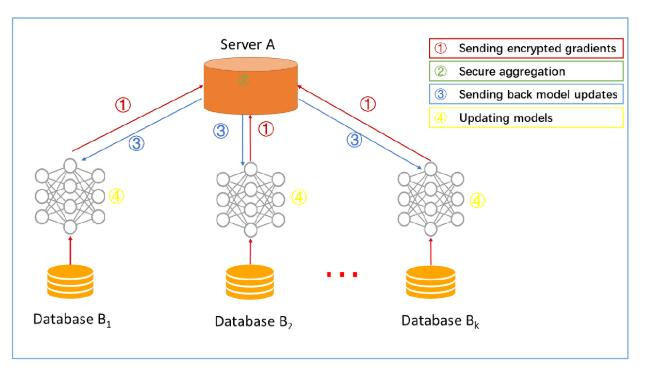
\includegraphics[width=0.9\textwidth]{Architecture_for_horizontal_FL_system.jpg}
    \caption{横向联邦学习的架构}
\end{figure}

\begin{enumerate}
\item 参与者本地计算训练梯度, 使用加密\citep{aono2017privacy}、差异隐私\citep{shokri2015privacy}或秘密共享技术屏蔽梯度\citep{bonawitz2017practical}, 并将屏蔽结果发送给服务器;
\item 服务器在没有关于任何参与者的学习信息的情况下执行安全聚合;
\item 服务器向参与者发送聚合的结果;
\item 参与者更新它们各自的模型具有解密的梯度.
\end{enumerate}

\paragraph{纵向联邦学习}
在两个数据集的用户重叠较多而用户特征重叠较少的情况下, 我们把数据集按照用户维度切分, 并取出双方用户相同而用户特征不完全相同的那部分数据进行训练.比如有两个不同机构, 一家是某地的银行, 另一家是同一个地方的电商.它们的用户群体很有可能包含该地的大部分居民, 因此用户的交集较大.但是, 由于银行记录的都是用户的收支行为与信用评级, 而电商则保有用户的浏览与购买历史, 因此它们的用户特征交集较小.纵向联邦学习就是将这些不同特征在加密的状态下加以聚合, 以增强模型能力的联邦学习.目前, 逻辑回归模型, 树型结构模型和神经网络模型等众多机器学习模型已经逐渐被证实能够建立在这个联邦体系上.


\begin{enumerate}
    \item  第三方C加密样本对齐[9-10].是在系统级做这件事, 因此在企业感知层面不会暴露非交叉用户.
    \item 对齐样本进行模型加密训练
    \begin{itemize}
        \item 由第三方C创建加密数据对, 并且向A和B发送公钥;
        \item A和B分别计算和自己相关的特征中间结果, 并加密交互, 用来求得各自梯度和损失;
        \item A和B分别计算各自加密后的梯度并添加掩码发送给C, 同时B计算加密后的损失发送给C;
        \item C解密梯度和损失后回传给A和B, A、B去除掩码并更新模型.
    \end{itemize}
\end{enumerate}
\paragraph{联邦迁移学习}
在两个数据集的用户与用户特征重叠都较少的情况下, 我们不对数据进行切分, 而可以利用 迁移学习\citep{pan2009survey}来克服数据或标签不足的情况.这种方法叫做联邦迁移学习.

比如有两个不同机构, 一家是位于中国的银行, 另一家是位于美国的电商.由于受到地域限制, 这两家机构的用户群体交集很小.同时, 由于机构类型的不同, 二者的数据特征也只有小部分重合.在这种情况下, 要想进行有效的联邦学习, 就必须引入迁移学习, 来解决单边数据规模小和标签样本少的问题, 从而提升模型的效果.

典型的跨设备联邦学习应用程序的数量级大小示意如表\ref{tab:sizes}.
 
\begin{table}
    \centering
    \renewcommand{\arraystretch}{1.2}
    \begin{tabular}{rl}    
    \toprule
    总群体大小 &  $10^6$--$10^{10}$ 设备\\
    为一轮训练选择的设备 & 50 -- 5000 \\
    参与训练一个模型的所有设备 & $10^5$--$10^7$  \\
    模型收敛的轮数 & 500 -- 10000 \\
    wall-colck训练的时间 & 1 -- 10 天 \\ 
    \bottomrule 
    \end{tabular}
    \caption{典型的跨设备联合学习应用程序的数量级大小}
    \label{tab:sizes}
\end{table}


数据中心的联邦学习和分布学习典型特性比较如表\ref{tab:characteristics}.
% Please add the following required packages to your document preamble:
% \usepackage[normalem]{ulem}
% \useunder{\uline}{\ul}{}
% Please add the following required packages to your document preamble:
%
 
\newpage

\newcolumntype{B}[1]{>{\arraybackslash}p{#1}}
\newcolumntype{P}[1]{>{\centering\arraybackslash}p{#1}}

% Widths shold be sum of the B{} widths below plus about 0.1in
\newcommand{\twocolright}[1]{\multicolumn{2}{p{4.1in}}{#1}}
\newcommand{\twocolleft}[1]{\multicolumn{2}{p{3.5in}}{#1}}
\newcommand{\twocolleftcenter}[1]{\multicolumn{2}{P{3.5in}}{#1}}


% \newgeometry{left=0.7in, right=0.7in, top=0.5in, bottom=0.8in}

\begin{table}[t]
    \begin{centering}
    \renewcommand{\arraystretch}{1.5}
    \begin{small}
    \begin{tabular}{@{}B{0.8in}B{1.6in}B{1.8in}B{2.2in}@{}}
    \toprule
     % The \hspaces are a nasty trick to get the line breaks where we want them.
     & \textbf{数据中心\mbox{分布式学习 }} & \textbf{Cross-silo\mbox{联邦学习 \hspace{1in}}} & \textbf{跨设备\mbox{联邦学习\hspace{1in}}} \\ 
    \midrule
    设置     
& 在大型但“扁平”的数据集 上训练模型.客户端是单个集群或数据中心中的计算节点.    & 在筒仓数据上训练模型. 客户是不同的组织(如医学或金融)或地理分布的数据中心.
& 客户是大量的移动或物联网设备. \\
    
    数据 \mbox{分布}
      & 数据是集中存储的, 可以在客户端之间转移和平衡.任何客户机都可以读取数据集的任何部分. 
      & \twocolright{\textbf{数据是在本地生成的, 并且仍然是去中心的.}  每个客户端存储自己的数据, 不能读取其他客户端的数据.数据不是独立或同分布的.} \\
    
    编排     
      &集中编排
      & \twocolright{\textbf{中央业务流程服务器/服务织训练},   但从不查看原始数据.} \\
    
    广域通信 \mbox{通信} 
      & 没有(一个数据中心/集群中完全连接的客户端)
      & \twocolright{星型拓扑, 其中hub中心节点表示协调服务提供者 (通常没有数据), 而spoke分支节点连接到客户端.} \\
    
      数据 \mbox{可用性 }
      & \twocolleftcenter{\rule[0.8mm]{.6in}{0.4pt}\ 所有的客户端几乎都是可用的.\ \rule[0.8mm]{.6in}{0.4pt}}
      & 在任何时间只有一小部分客户端可用, 通常是按日或其他变化的. \\
      分布范围
      &通常有1 - 1000个客户.
      &通常有2 - 100个客户.
      & 大规模并行, 高达$10^{10}$个客户端.
      \\
      
      主要\mbox{瓶颈}
      & 和计算通常是数据中心的瓶颈, 在那里可以假设有非常快的网络.
      & 可能是计算或通信. 
      & 沟通通常是主要的瓶颈, 尽管它取决于任务.通常, 跨设备联邦计算使用wi-fi或较慢的连接.
      \\
      
      可寻址能力
      & \twocolleft{每个客户端都有一个身份或名称, 允许系统专门访问它.}
      &客户端不能被直接索引.(即, 不使用客户端标识符).
      \\
      
      客户端\mbox{有状态性}
      & \twocolleft{有状态的----每个客户端可以携带状态从一轮到另一轮, 参与每一轮的计算.
      }
      &无状态---每个客户端可能只参与一次任务, 因此通常假设在每一轮计算中都有一个从未见过的客户端新样本.
      \\
      
      客户端\mbox{可靠性}
      & \twocolleftcenter{\rule[0.8mm]{1.0in}{0.4pt} \ 相对较少的失败.
      \ \rule[0.8mm]{1.0in}{0.4pt} }
      &高度不可靠----参与一轮计算的客户端中有5\%或更多可能会失败或退出(例如, 当违反了电池、网络或闲置要求时, 设备就不合格了).
      \\
      
      数据分区轴
      &数据可以在客户端之间任意分区/重新分区.
      &分区是固定的.可以是分区示例(水平)或分区特性(垂直).
      &固定分区的例子(横向).\\ 
    
    \bottomrule
    \end{tabular}
    \end{small}
    \caption{典型特征联邦学习设置与数据中心的分布式学习(例如\citep{dean2012large}). 跨设备和cross-silo跨孤井联邦学习是联邦学习领域的两个例子, 但并不是详尽的.}
    \label{tab:characteristics}
    \end{centering}
    \end{table}
  
    \subsubsection{联邦学习中模型的生命周期}
    \begin{figure}[ht]
        \setlength{\abovecaptionskip}{0.1cm}
        \centering    
        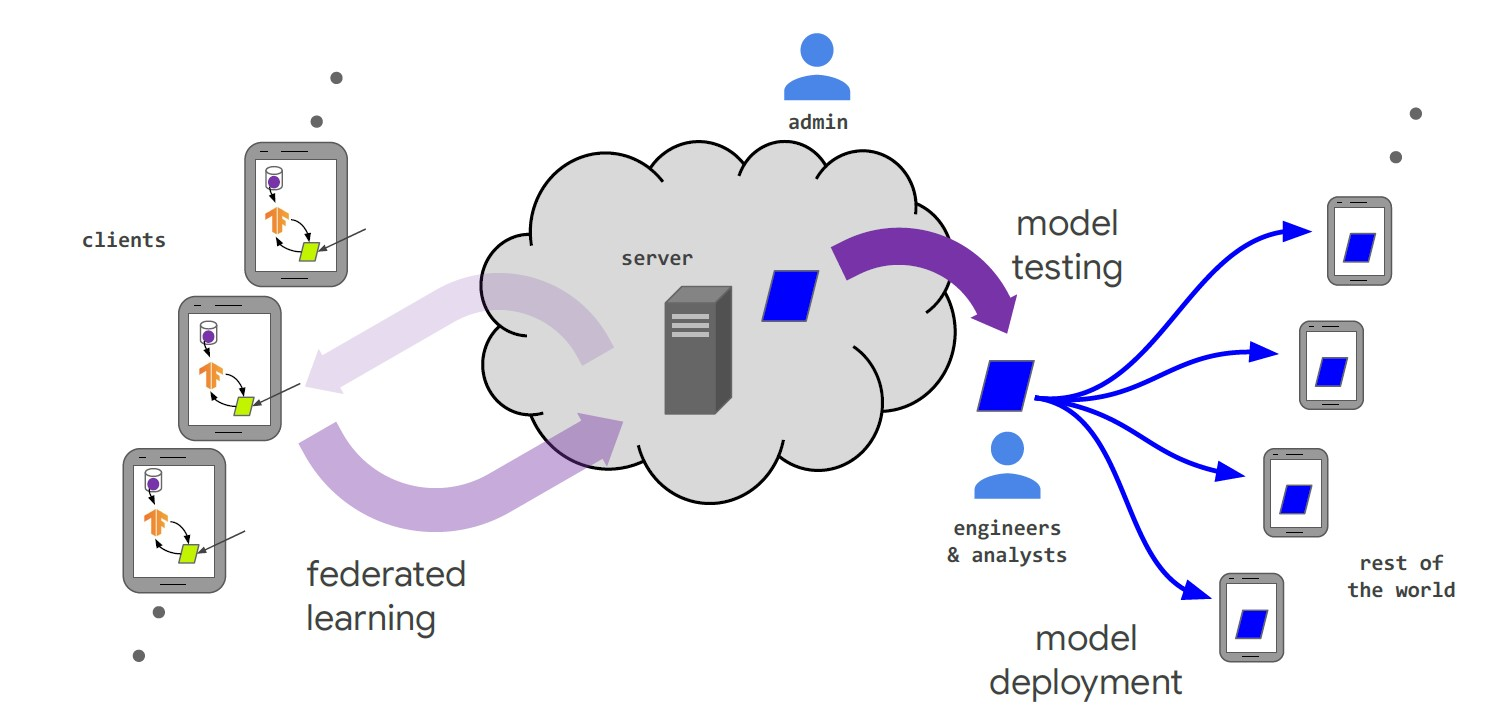
\includegraphics[width=0.6\textwidth]{life_circle.jpg}
        \caption{联邦学习中模型的生命周期}
    \end{figure}
在联邦学习过程中, 模型的生命周期通常由为特定应用程序开发模型的模型工程师驱动.例如, 自然语言处理领域的专家可以开发用于虚拟键盘的下一个单词预测模型.图1显示了主要组件和参与者.在高层, 一个典型的工作流程是:
\begin{enumerate}
\item	\textbf{问题识别:}\ 模型工程师识别出一个需要用FL解决的问题.
\item	\textbf{客户端插装:} \ 如果需要, 客户端(例如在移动电话上运行的应用程序)被插装到本地存储(有时间和数量限制)必要的训练数据.在许多情况下, 应用程序已经存储了这些数据(例如, 一个文本消息应用程序必须存储文本消息, 一个照片管理应用程序已经存储了照片).然而, 在某些情况下, 可能需要维护额外的数据或元数据, 例如用户交互数据来为监督学习任务提供标签.
\item	\textbf{仿真原型(可选):} \ 模型工程师可以在一个使用代理数据集的FL仿真中原型模型架构和测试学习超参数.
\item	\textbf{联邦模型训练:} \ 启动多个联邦训练任务来训练模型的不同变体, 或使用不同的优化超参数.
\item	\textbf{(联邦)模型评估:} \ 在任务得到充分训练(通常是几天, 见下文)之后, 分析模型并选择合适的候选者.分析可能包括在数据中心的标准数据集上计算的度量, 或者联合评估, 在联合评估中, 模型被推送到指定的客户端, 以对本地客户端数据进行评估.
\item	\textbf{部署:} \ 最后, 一旦选择了一个好的模型, 它通过一个标准模型发布过程, 包括人工质量保证, 在线A/B测试(通常通过使用新模型在一些设备和其他设备来比较他们的上一代模型体内性能), 并分阶段推出(以便于发现表现差的行为并且在影响太多的用户之前回退).模型的特定启动过程由应用程序的所有者设置, 通常与模型的训练方式无关.
\end{enumerate}
 
\subsubsection{典型的联邦训练过程}
我们现在考虑一个FL训练模板, 它包含McMahan等人\citep{mcmahan2016communication}和许多其他人的联邦平均算法;同样, 可能会有变化, 但这提供了一个共同的起点.
服务器(服务提供商)通过重复以下步骤来编排训练过程, 直到训练停止(由监控训练过程的模型工程师决定):


\begin{enumerate}
\item 客户端选择:服务器从一组满足资格要求的客户端取样.例如, 为了避免影响设备的用户, 移动电话可能只有在接入无线网络并处于空闲状态时才会登录到服务器.
\item 广播:选定的客户端从服务器下载当前模型的权值和一个训练程序(例如一个TensorFlow图表[6]).
\item 客户端计算:每个选择的设备通过执行训练程序在本地计算对模型的更新, 例如可以在本地数据上运行SGD(如联合平均).
\item 聚合:服务器收集设备更新的聚合.为了提高效率, 一旦有足够数量的设备报告了结果, 掉队者可能会被丢弃.此阶段也是许多其他技术的集成点, 稍后将讨论这些技术, 可能包括:用于增加隐私的安全聚合、用于提高通信效率的聚合的有损压缩, 以及用于差异隐私的噪声添加和更新裁剪.
\item 模型更新:服务器根据从参与当前轮的客户机计算的聚合更新, 在本地更新共享模型.
\end{enumerate}
表2给出了移动设备上典型的联邦学习应用程序所涉及的数量的典型数量级大小.

%%
%这一部分你可以根据你对论文的理解进一步提炼.关于该问题目前研究的进展是什么?目前已有哪些工作?这些工作之间的发展脉络是什么?

\subsection{联邦学习研究} 

联邦学习和完全去中心化学习的主要区别比较如表\ref{tab:decentralized}.
注意使用联邦学习, 去中心化学习可以进一步划分为不同的用例.
\begin{table}
    \begin{centering}
    \renewcommand{\arraystretch}{1.5}
    \begin{tabularx}{\textwidth}{lXX}
    \toprule
           & \textbf{联邦学习} & \textbf{完全去中心化(端对端学习)} \\
    \midrule  
编排
&中心业务流程服务器或服务组织训练, 但从不查看原始数据.
&没有集中的业务流程.
\\
广域通信
& hub-and-spoke拓扑, 其中hub表示协调服务提供者(通常没有数据), 而spoke节点连接到客户端.
&点对点拓扑, 可能是动态连接图.
\\ 
    \bottomrule
    \end{tabularx}
    \caption{联邦学习和完全去中心化学习的主要区别}
    \label{tab:decentralized}
    \end{centering}
\end{table}
 
\subsubsection{Cross-soli联邦学习} 
与跨设备联合学习的特征相反,  跨孤井Cross-Silo联邦学习在总体设计的某些方面非常灵活.许多组织如果只是想共享训练模型, 而不想分享数据时, cross-silo设置是非常好的选择.Cross-Silo 联邦学习的设置主要有以下几个要点:数据分割、激励机制、.差异隐私、张量因子分解.


分割学习(Split Learning):分割学习的关键思想是在客户端和服务器之间执行基于每层的分割模型, 并应用于训练和推理.分裂学习最简单配置是每个客户端计算通过深层网络前向传递, 然后切割层的输出, 即粉碎数据被发送到另一个服务器或客户端, 然后由此服务器或客户端完成剩余的计算.这意味着让不共享的数据发生前向传播;最后可以以类似的方式将梯度从其最后一层反向传播到切割层.注意此过程会一直持续到收敛.
\begin{figure}[ht]
    \centering    
    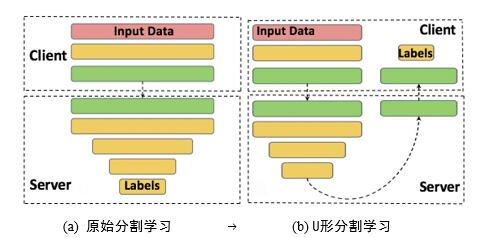
\includegraphics[width=0.6\textwidth]{split_learning.jpg}
    \caption{分割学习}
\end{figure}


分割学习(Split learning)的关键思想, 与之前着重于数据分区和通信模式的设置相比, 它是在客户端和服务器之间按层划分执行模型, 这对于训练和推理都是一样的.
如图所示:(a)在普通拆分学习的设置, 原始数据不会传输;(b)在U-形拆分学习的设置, 在客户端和服务器实体之间原始数据和标签不会传输.



\subsubsection{算法挑战}



联邦学习的核心是谷歌在其论文\cite{mcmahan2016communication}中引入的联邦平均算法\cite{alg:fedavg}。
 

   \begin{algorithm}[t]
    \begin{algorithmic}
    \State \textbf{Server executes:}
       \State initialize $w_0$
       \FOR{each round $t = 1,  2,  \dots$} 
       \hspace{1em} \State $m \leftarrow \max( C\cdot K,  1)$
          \State $S_t \leftarrow$ (random set of $m$ clients)
           \FOR{each client $k \in S_t$ \textbf{in parallel}}
            \State $w_{t+1}^k \leftarrow \text{ClientUpdate}(k,  w_t)$ 
           \State $w_{t+1} \leftarrow \sum_{k=1}^K \frac{n_k}{n} w_{t+1}^k$ \\

     \State {\textbf{ClientUpdate}($k,  w$):}\ \ \  // \emph{Run on client $k$}
      \State $\mathcal{B} \leftarrow$ (split $\mathcal{P}_k$ into batches of size $\lbs$)
       \FOR{each local epoch $i$ from $1$ to $ \lepochs$}
      \FOR{batch $b \in \mathcal{B}$}
         \State $w \leftarrow w - \eta \nabla \ell(w; b)$
       \State return $w$ to server
    \end{algorithmic}
    \caption{FederatedAveraging. The $K$
      clients are indexed by $k$; $\lbs$ is the local minibatch size, 
      $\lepochs$ is the number of local epochs,  and $\eta$ is the learning
      rate.} 
    \label{alg:fedavg}
    \end{algorithm}
     
    \begin{description}
        \item[Step1:] 选择成员的一个随机子集(称为客户机)以同步方式从服务器接收全局模型。
        \item[Step2:] 每个选择的客户端使用其本地数据计算一个更新的模型。
        \item[Step3:] 模型更新从选择的客户端发送到服务器。 
        \item[Step4:] 服务器聚合这些模型(通常通过平均)来构建一个改进的全局模型。 
    \end{description}

子集选择步骤是谷歌最初应用联邦学习的环境所必需的:\textbf{基于在其Android生态系统中通过数百万部手机收集的数据}。这种学习序列的一种变体出现在之后的论文中, 包括发送梯度更新到服务器, 而不是实际的模型权重本身。通常, 在各方之间不传输任何原始数据, 只传输与模型相关的更新。\textbf{边缘计算}在这里体现出作用。
 
在机器学习分散方案的现实可用性问题上, 许多重要的算法问题仍然没有解决.有些问题类似于使用中央服务器进行联合学习的特殊情况, 而其他挑战则是完全分散或不信任的额外副作用.如
\begin{itemize}
    
\item 网络拓扑结构和异步性对去中心化SGD的影响
\item 本地更新对与中心化SGD
\item 个性化和信任机制
\item 梯度压缩和量化方法
\end{itemize}

\paragraph{}
 
    \subsubsection{实际挑战}

今天的区块链平台数据在默认情况下, 可能会阻止用户参与联邦分割学习.

解决方案:
为了防止参与节点利用单独提交的模型更新, 可以使用现有的安全聚合协议.

为了防止任何客户机试图重建另一个客户的私人数据利用全球模型, 客户级差分隐私[290]已被提议用于FL.客户级差分隐私是通过在聚合的全局模型上添加随机高斯噪声来实现的, 该噪声足以隐藏任何单个客户端的更新.

\paragraph{推理攻击} 联邦学习的动机是保护客户拥有的数据的隐私。即使没有公开实际数据, 也可以利用重复的模型权重更新来揭示对数据而言不是全局的而是特定于各个贡献者的属性。可以在服务器端以及(其他)客户端端执行此推断。通常引用的对策是使用差异隐私来减轻这种风险。

\paragraph{模型中毒Model Poisoning}。一些研究人员研究了使客户误导后门功能或进行Sybil攻击以毒害全局模型的可能性。
 \textbf{Sybil} 攻击:允许客户端加入和离开的系统容易受到sybil攻击, 在这种攻击中, 对手通过使用多个串通的别名加入一个系统来获得影响力。
\begin{figure}[t]
    \centering    
    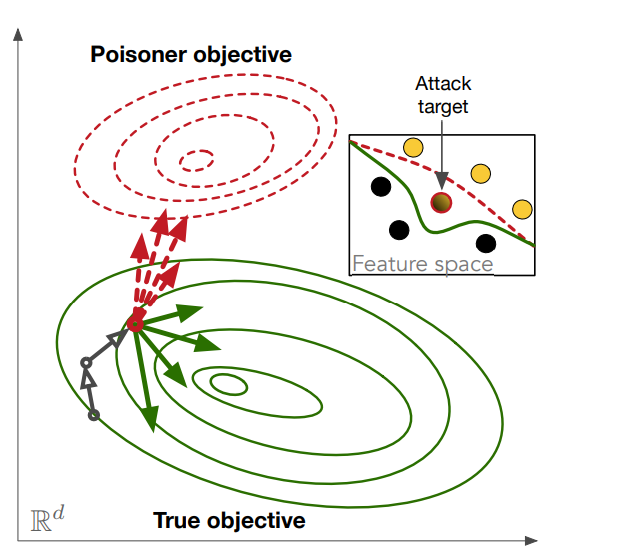
\includegraphics[width=0.6\textwidth]{poisoninginSGD.png}
    \caption{Targeted poisoning attack in SGD. 红色点的矢量是Sybil的贡献, 推动模型走向一个中毒的目标。坚实的绿色载体是由诚实的客户贡献的, 推动到达真正的目标。    }
\end{figure}
为了有效应对此类攻击, 必须考虑Sybil检测的额外开销。
\section{提高效率和效果}

提高联邦学习的效率和效果
\begin{enumerate}
    \item 开发更好的优化算法;为不同的客户提供不同的模型;
    \item 使ML任务, 如超参数搜索、架构搜索和调试在FL上下文中更容易;
    \item 提高沟通效率
\end{enumerate} 

\subsection{挑战一--联邦学习中的非独立同分布数据}
现有的机器学习任务默认训练数据遵循独立同分布, 神经网络常见算法一般都将数据遵循IID的假设作为其推导的一部分.但是, 在真实世界中样本数据相关性几乎无处不在, 非同源数据/标签的分布也可能具有不同的概率分布, 这些数据都遵循非独立同分布.
在一些场景中, 直接应用已有机器学习算法基于 Non-IID 数据完成模型训练, 由于算法本身的先进性训练结果仍然较好.但对于某些应用场景, 基于现有的机器学习算法和框架, 使用 Non-IID 数据训练会出现意想不到的负面效果, 比如模型准确度低、模型无法收敛等.
比较常见的需要处理 Non-IID 数据问题的应用场景包括:异常检测(Outlier Detection)、生物医学应用(Medical Data)、联邦学习 (Federated Learning).

在联邦学习的应用场景中, 各个设备上的数据是由设备/用户独立产生的, 不同设备/用户的非同源数据具有不同的分布特征, 而每一个设备在进行本地学习的时候, 所学习的训练数据是 Non-IID 的.因此研究提升 Non-IID 数据的学习效率, 对于联邦学习具有重要意义.联邦学习允许用户在不需要集中存储数据的情况下, 从本地存储的数据中共同获得共享模型的好处.客户端的本地数据通常基于特定用户对移动设备的使用, 因此任何特定用户的本地数据集都不能代表总体分布.


依赖和非同质性的最常见来源是对应于特定用户、特定地理位置和/或特定时间窗口的每个客户机.这种分类法与数据集移位的概念有密切的关系,  其中研究了训练分布和测试分布之间的差异;这里, 我们考虑每个客户机上数据分布的差异.

以下, 考虑一个监督任务特征x和y标签.联邦学习的的统计模型, 给出学习包括两个层次的抽样:访问一个数据需要首先采样一个客户$i\sim Q$, 客户可用的分布, 然后画一个例子$(x,  y) \sim P_i(x,  y)$从客户机的本地数据分布.

当引用联合学习中的非iid数据时, 这通常是指Pi和Pj对于不同的i和j客户机的差异.然而, 值得注意的是, 分布$Q$和$Pi$可能会随着时间的变化而变化, 从而引入另一个“non-iidness”维度.

为了完整性: 单个设备上的数据集,  独立性在局部也可能会被破坏, .例如, 视频中连续的帧是高度相关的.客户端内部相关性的来源通常可以通过\textbf{局部变换}来解决.

\paragraph{非同质的客户端分布}
数据偏离同分布的方式\citep{hsieh2019non},     $P_i \neq P_j$ 代表不同客户端 $i$ and $j$. 用 $P_i(y | x) P_i(x)$ and $P_i(x | y) P_i(y) $重写$P_i(x,  y)$, 这样可以更精确地描述不同.
\begin{description}
\item[特征分布倾斜] 即使$P(y, j, x)$相同,  $P_i(x)$的边际分布在不同的客户端之间也可能不同
\item[标签分布倾斜] 即使$P(x,  j,  y)$是相同的, $P_i(y)$的边际分布在不同的客户端可能是不同的.
\item[标签相同, 特征不同] 即使 $P(y)$相同,  $Pi(x, j, y)$的条件分布在不同的客户机上也可能不同. 
\item[特征相同, 标签不同] 即使$P(x)$是相同,  条件分布$Pi(y, j, x)$在不同的客户端可能不同, .
\item[数量倾斜或不平衡]不同客户端拥有不同数量数据. 
\end{description}

此外, 不同的non-iid方式可能需要制定不同的应对策略.例如, 由于假定$P(y | x)$是常见的, 所以在特征分布倾斜的情况下, 至少在原则上详细说明了这个问题, 并且训练一个学习$P(y | x)$的全局模型可能是适当的.当相同的特性映射到不同客户端上的不同标签时, 可能需要训练某种形式的个性化模型.

\paragraph{违反独立性}
在训练过程中, 一旦分布Q发生变化, 就会出现违反独立性的情况.一个例子是跨设备FL中设备通常需要满足资格要求才能参加训练.设备通常在夜间本地时间满足这些要求(当它们更有可能在充电、使用免费wi-fi和空闲时), 因此设备可用性可能存在明显的昼夜变化模式.此外, 由于当地时间与经度直接相关, 这就在数据来源中引入了很强的地理偏差.Eichner等人[151]描述了这个问题和一些缓解策略, 但仍有许多悬而未决的问题.

\paragraph{数据集偏移}
Q和P分布的时间依赖性可能会引入经典意义上的数据集偏移(训练分布和测试分布之间的差异).此外, 其他条件可能会使有资格训练联合模型的客户端集合不同于将部署该模型的客户端集合.例如, 训练可能需要比推理所需内存更多的设备. 


%将处理数据集的技术转换为联邦学习是另一个有趣的开放问题.
\subsubsection{解决non-IID Data 问题的策略}
联合学习的最初目标是在客户端数据集的联合上训练单个全局模型, 但对于non-iid数据, 这一目标更难实现.一种自然的方法是\textbf{修改现有的算法(例如通过不同的超参数选择)或开发新的超参数}以更有效地实现这一目标.
对于某些应用程序, 可能需要增加数据以使跨客户机的数据更加相似.一种方法是\textbf{创建一个可以全局共享的小数据集}.该数据集可能来自一个公开可用的代理数据源, 一个独立于客户端数据的不隐私敏感的数据集, 或者可能是原始数据的提炼.客户目标函数的异构性使得如何构建目标函数的问题变得更加重要——现在已经不清楚是否对所有示例都同等看待.
multi-model
替代选择包括\textbf{限制来自任何一个用户的数据贡献}, 并\textbf{在客户端之间引入公平}的概念.但是, 如果我们能够在每个设备上的本地数据上运行训练(这对于全局模型的联合学习是必要的), 那么训练单个全局模型是否是正确的目标呢? 
在许多情况下, 最好使用单个模型, 例如为了向没有数据的客户端提供模型, 或者为了在部署之前允许手工验证和质量保证.然而, 由于本地训练是可能的, 因此每个客户都有一个定制的模型是可行的.这种方法可以把非iid问题从一个bug变成一个特性, 几乎是字面上的意思——因为每个客户端都有自己的模型, 客户端的身份有效地参数化了模型, 使一些病态但退化的非iid分布变得微不足道.例如, 如果对于每一个$i,  Pi(y)$仅在一个标签上有支持, 那么找到一个高精度的全局模型可能是非常具有挑战性的(特别是当x的信息相对不足时), 但是训练一个高精度的局部模型是不重要的(只需要一个恒定的预测). 
除了解决不相同的客户端之外, 使用多个模型还可以解决由于客户端可用性变化而导致的独立性违背问题.
\subsection{联邦学习的优化算法}
在典型的联邦学习任务中, 目标是学习单个全局模型, 该模型最小化整个训练数据集上的风险函数, 即所有客户机的数据联合.联邦优化算法和分布式训练方法之间的主要区别是, 对于优化, non-iid和不平衡数据、有限的通信带宽、不可靠的和有限的设备可用性是特别突出的.

FL设置中, 设备的总数是巨大的(例如跨移动设备), 这就要求算法每轮只需要少量的客户端参与(客户端抽样).此外, 每个设备在给定模型的训练中可能只参与一次, 因此无状态算法是必要的.这就排除了直接应用在数据中心环境中非常有效的各种方法, 例如ADMM之类的有状态优化算法, 以及根据前几轮遗留的压缩错误修改更新的有状态压缩策略.
联邦学习算法的另一个重要的实际考虑是与其他技术的可组合性.优化算法不会在生产部署中单独运行, 但需要与其他技术相结合, 如加密的安全聚合协议、差异隐私(DP)和模型和更新压缩.这些技术可以应用于原语“选中求和客户”和“广播选择客户”, 所以表达这些原语方面的优化算法提供了一个宝贵的关注点分离, 但也可能排除某些技术, 如异步应用更新.
最常见的一种优化方法对于联邦学习是联邦平均算法\citep{mcmahan2016communication}, 采用local-update或parallel SGD.这里, 每个客户端运行在本地一些SGD步骤, 然后更新本地模型平均形成协调服务器上更新全局模型.伪代码在算法1中给出.执行本地更新并减少与中央服务器的通信频率, 解决了尊重数据位置约束和移动设备客户端有限通信能力的核心挑战.然而, 从优化理论的角度来看, 这类算法也带来了一些新的算法挑战. 开发专门针对联邦学习设置特征的新算法仍然是一个重要的开放问题.
\begin{figure*}[ht]
    \setlength{\abovecaptionskip}{0.1cm}
    \centering    
    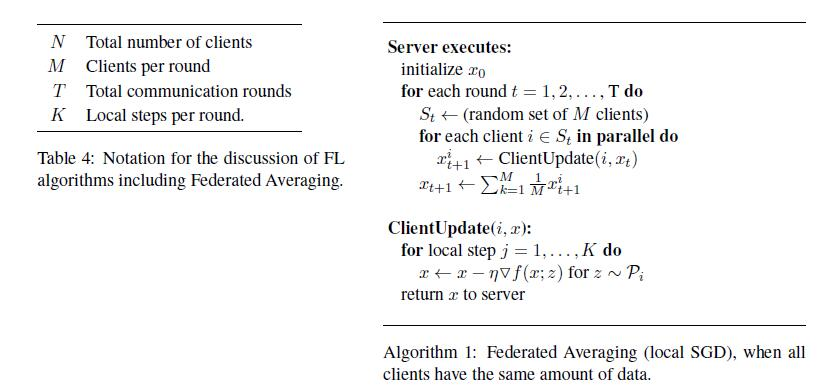
\includegraphics[width=0.9\textwidth]{Federated_Averging.jpg}
    \caption{联邦平均算法}
\end{figure*}

\subsubsection{ IID数据集的优化算法和收敛速度}

虽然可以对正在优化的每个客户端函数进行各种不同的假设, 但最基本的划分是假设IID和非IID数据.在形式上, 在客户端拥有IID数据意味着用于客户端本地更新的每一小批数据在统计上与从整个训练数据集中(客户端所有本地数据集的联合)一致绘制的样本(带有替换)相同.由于客户独立地收集他们自己的培训数据, 这些数据在大小和分布上都有所不同, 而且这些数据不与其他客户或中心节点共享, 因此IID的假设在实践中几乎不可能成立.然而, 这个假设极大地简化了联邦优化算法的理论收敛分析, 并建立了一个基线, 可以用来理解非IID数据对优化率的影响.因此, 自然的第一步是了解IID数据案例的优化算法.
 
% Communication-Efficient Learning of Deep Networks from Decentralized Data
% \citep{mcmahan2016communication}

% Federated Learning with Non-IID Data 
% \citep{zhao2018federated}

\section{保护用户数据的隐私}
 面向隐私保护的机器学习(Privacy-Preserve Machine Learnin, PPML), 指的是使用了保护用户隐私和数据安全的防御技术的机器学习。其中有以下几种著名方法。\citep{ppmlmancuso}
 \begin{itemize}
     \item 
 安全多方计算(Secure Multiparty Computation,  MPC)
 \item 
 供隐私保护模型训练和预测使用的 同态加密方法(Homomorphic Eneryption,  HE )
 \item 
 用于防止数据泄器的差分隐私 iferntial Piaey, DP) 方法。
 \end{itemize}
 
 \subsection{隐私保护技术}
 \subsubsection{安全多方计算}
 安全多方计算起初是应对安全两方问题(百万富翁问题)。 
  
2.4隐私保护技术
包括三种方法, 分别是安全多方计算、同态加密和差分
本节讨论隐私保护技术, 
隐私。
2.4.1安全多方计算
安全多方计算最初是针对一个安全两方计算问题, 即所谓的“百万富翁问题”:两个争强好胜的富翁 Alice 和 Bob 在街头相遇, 如何在不暴露各自财富的前提下比较出谁更富有?\citep{scyao1982}

被提出的, 并于1982年由姚期智提出和推广。在安全多方计算中, 目的是协同地从每一方的隐私输人中计算函数的结果, 而不用将这些输入展示给其他方。
\paragraph{数学描述}
有 $n $个参与者 $P_1, P_2, ...P_n$, 要以一种安全的方式共同计算一个函数, 这里的安全是指输出结果的正确性和输入信息、输出信息的保密性。具体地讲, 每个参与者 $P_1$, 有一个自己的保密输入信息 $X_i$, $n $个参与者要共同计算一个函数 $f(X_1, X_2, ... , X_n)=(Y_1, Y_2,  ... , Y_n)$,  计算结束时, 每个参与者 $P_i $只能了解 $Y_i$,  不能了解其他方的任何信息。

\begin{itemize}
    \item  输入隐私性:安全多方计算研究的是各参与方在协作计算时如何对各方隐私数据进行保护, 重点关注各参与方之间的隐私安全性问题, 即在安全多方计算过程中必须保证各方私密输入独立, 计算时不泄露任何本地数据。
\item    计算正确性:多方计算参与各方就某一约定计算任务, 通过约定MPC协议进行协同计算, 计算结束后, 各方得到正确的数据反馈。
    \item     去中心化:传统的分布式计算由中心节点协调各用户的计算进程, 收集各用户的输入信息, 而安全多方计算中, 各参与方地位平等, 不存在任何有特权的参与方或第三方, 提供一种去中心化的计算模式。
\end{itemize}

\begin{enumerate}
    \item 参与方个数区分
    \item 计算场景区分
\end{enumerate}

主流的两方计算框架的核心是用了混淆电路(Garbled Circuit, 简称GC)和不经意传输(Oblivious Transfer)这两种密码学技术
通用的多方安全计算框架可以让多方安全地计算任何函数或某类函数的结果。自1986年姚期智提出第一个通用的多方安全计算框架(常被称为Yao’s GC, 即姚氏加密电路)以来, 30多年间已经有BMR、GMW、BGW、SPDZ等多个多方安全计算框架陆续提出。
\citep{GenExchsecretyao1986}
\paragraph{不经意传输:}
发送方将潜在的许多信息中的一个传递给接收方, 但是对于已传输的信息(如果有的话)则保持忽略。


\paragraph{n取1 的不经意传输:}设A方有一个输入表 $(x_1..., x_n)$作为输入, 
B方有$i \in 1,  \dots , n$作为输入。n取1的不经意传输是一种安全多方计算协议, 其中
A不能学习到关于$i$的信息, B只能学习到$x_i$
\subsubsection{同态加密}
同态加密指, 对明文进行环上的加法和乘法运算再加密, 与加密后对密文进行相应的运算, 结果是等价的。
全同态加密是指同时满足加同态和乘同态性质, 可以进行任意多次加和乘运算的加密函数。用数学公式来表达, 即$Dec(f(En(m_1), En(m_2), …, En(m_k)))=f(m_1, m_2, …, m_k)$, 或写成:$f(En(m_1), En(m_2), …, En(m_k))=En(f(m_1, m_2, …, m_k))$, 如果f是任意函数, 称为全同态加密。
% \cite{encrygoldwass1982}
\paragraph{加法同态}, 如果存在有效算法$\odot$$, E(x+y)=E(x)\odot E(y)$或者$ x+y=D(E(x)\odot E(y))$成立, 并且不泄漏 x 和 y。
\paragraph{乘法同态}, 如果存在有效算法, $E(x \times y)=E(x) \dot E(y)$或者$ xy=D(E(x) E(y))$成立, 并且不泄漏 x 和 y。



\subsubsection{差分隐私} 
差分隐私是为了允许研究者在不泄露个体信息(用户隐私)的前提下对一个数据集的整体进行分析而研究出的加密手段。\cite{DPDwork2008}
设想一个受信任的机构持有涉及众多人的敏感个人信息(例如医疗记录、观看记录或电子邮件统计)的数据集, 但想提供一个全局性的统计数据。这样的系统被称为统计数据库。但是, 提供有关数据的综合性统计也可能揭示一些涉及个人的信息。事实上, 当研究人员链接两个或多个分别无害化处理的数据库来识别个人信息时, 各种公共记录匿名化的特殊方法都失效了。而差分隐私就是为防护这类统计数据库脱匿名技术而形成的一个隐私框架。

令 $\varepsilon$ 为正实数, $\mathcal{A}$是将数据集作为输入的随机算法(代表持有数据的受信方的行为)。让 $\textrm{im}\mathcal{A}$表示图像的$\mathcal {A}$。对于所有数据集$D_{1}, D_{2}$, 
算法$\mathcal{A}$ 提供 $\epsilon-$差分隐私, 在单个元素(即一个人的数据)以及$\mathcal{A}$的所有子集上有所不同 $S$. 
$$ Pr [ \mathcal{A}(D_1) \in S ] \leqslant \exp(\epsilon c) \cdot Pr [ \mathcal{A(D_2)} ] \in S  $$
其中用概率代替算法的随机性。 
  
\paragraph{劣势:}由于对于背景知识的假设过于强(在加噪音的时候需要使用与原数据分布比较类似的噪音函数, 而这一条件就限制了大多数数据其实不满足插分隐私的使用条件), 需要在查询结果中加入大量的随机化, 导致数据的可用性急剧下降。特别对于那些复杂的查询, 有时候随机化结果几乎掩盖了真实结果。
\paragraph{应用}
\begin{itemize}
    \item Google的RAPPOR, 用于遥测, 例如了解统计劫持用户设置的恶意软件(RAPPOR's \item open-source implementation)
    \item Google, 分享历史流量统计信息。
    \item 2016年6月13日, 苹果公司宣布其在iOS 10中使用差异隐私, 以改进其虚拟助理和建议技术,  
    \item 在数据挖掘模型中使用差异隐私的实际表现已有一些初步研究。\citep{FLETCHER201716}
    \item 2020年LinkedIn, 用于广告客户查询
\end{itemize}
\section{预备知识}

%% 这儿总结一些比较重要的数学概念、定理等.
\subsection{梯度下降}
\subsubsection{随机梯度下降Stochastic gradient descent}
随机梯度下降(通常缩写SGD)是一种迭代方法用于优化的目标函数与合适的光滑性质(例如可分化或subdifferentiable).它可以被看作是随机逼近的梯度下降优化, 因为它取代了实际梯度(从整个计算数据集通过其估计值(从数据中随机选择的子集计算)).特别是在大数据应用中, 这减轻了计算负担, 实现更快的交易迭代, 但收敛速度略低. 
\begin{algorithm}  
    \caption{ Stochastic  General decent method}  
    \begin{algorithmic}
          
\State Choose an initial vector of parameters  w and learning rate  $\eta$ .
Repeat until an approximate minimum is obtained:
\begin{itemize}
    \item Randomly shuffle examples in the training set.
    \item For $  i=1, 2, ..., n$,  do:
    $w:=w-\eta \nabla Q_{i}(w)$ 
\end{itemize}
    \end{algorithmic}  
   \end{algorithm}  
\subsubsection{ADMM 交替向量乘子法}
ADMM也是增广拉格朗日函数, 只是由一个变量变成两个变量
$$L(x, z;\lambda)= f(x) + g(z) + \lambda ^T(Ax + Bz - c) + \rho/2 * ||Ax + Bz -c ||^2$$
固定其中两个变量, 去更新第三个变量的值
$step1: x^{k+1} = arg \min_x L(x, z^k, \lambda^k) \\
step2: z^{k+1} = arg min_z L(x^{k+1}, z, lambda^k) \\
step3: \lambda ^ {k+1} = \lambda^k + \rho (Ax + Bz - c) \\$
于是问题就变化为了如何求解 $arg min_x L$
\subsubsection{decentralized SGD去中心化 SGD}

.......

Decentralized Federated Learning via SGD over Wireless D2D Networks (H Xing,  O Simeone,  S Bi)

\subsection{张量分解}
张量(tensor)是一个多维的数据存储形式, 数据的的维度被称为张量的阶.它可以看成是向量和矩阵在多维空间中的推广, 向量可以看成是一维张量, 矩阵可以看成是两维的张量.
\subsubsection{CP分解}
将高维的张量分解成为Rank-One Tensors的和.
$X \approx [ \!  [ \mathbf{A, B, C} ]\!] \equiv \sum_{r=1}^{R}a_r \circ b_r \circ c_r$

这里$\circ$指的是外积.
\subsubsection{Tucker 分解  }

Tucker分解将张量分解为一组矩阵和一个小的核心张量.

 $X = G \times_1 A^{(1)} \times_2  A^{(2)} \dots \times_N A^{(N)}= [\! [  G:A^{(1)},  A^{(2)},  A^{(N)}   ] \! ] $

\subsection{Dataset shift 数据集偏移}
数据集偏移是指训练和测试分布不同时的情况.
数据集偏移主要发生在有监督的机器学习范式和半监督学习的混合范式内.
数据集移位的问题可能源于利用输入特征的方式, 选择训练和测试集的方式, 数据稀疏性, 由于非平稳环境而导致的数据分布移位, 以及源于各层内激活模式的变化.深度神经网络.
数据集移位的表现形式:协变量移位、先验概率转移、概念转变、内部协变量移位(协变量移位的重要子类型)

\subsubsection{有状态和无状态}
有状态就是有数据存储功能.有状态对象(Stateful Bean), 就是有实例变量的对象 , 可以保存数据, 是非线程安全的.在不同方法调用间不保留任何状态.

无状态就是一次操作, 不能保存数据.无状态对象(Stateless Bean), 就是没有实例变量的对象.不能保存数据, 是不变类, 是线程安全的.
 
\subsection{激活函数}
激活函数在神经元中非常重要的.为了增强网络的表示能力和学习能力, 激活函数需要具备以下几点性质:
\begin{enumerate}
\item 连续并可导(允许少数点上不可导)的非线性函数.可导的激活函数可以直接利用数值优化的方法来学习网络参数.
\item 激活函数及其导函数要尽可能的简单, 有利于提高网络计算效率.
\item 激活函数的导函数的值域要在一个合适的区间内, 不能太大也不能太小, 否则会影响训练的效率和稳定性.
\end{enumerate}
\subsubsection{Sigmoid型函数}
常用的Sigmoid 型函数有Logistic 函数和Tanh 函数.
\paragraph{Logistic函数}
$$\sigma(x)=\frac{1}{1+\exp(-x)}$$
和感知器使用的阶跃激活函数相比, Logistic 函数是连续可导的, 
装备了Logistic激活函数的神经元具有以下性质:
\begin{enumerate}
    \renewcommand{\labelenumi}{(\theenumi)}
 \item 其输出直接可以看作概率分布, 使得神经网络可以更好地和统计学习模型进行结合. 
 \item 其可以看作一个软性门(Soft Gate), 用来控制其他神经元输出信息的数量.
\end{enumerate}

\textbf{优点}:
\begin{enumerate}
    \renewcommand{\labelenumi}{(\theenumi)}
\item 便于求导的平滑函数;
\item 能压缩数据, 保证数据幅度不会有问题;
\item 适合用于前向传播.
\end{enumerate}

\textbf{缺点}:
\begin{enumerate}
    \renewcommand{\labelenumi}{(\theenumi)}
    \item 容易出现梯度消失的现象 
   \item Sigmoid的输出不是0均值 的:这会导致后层的神经元的输入是非0均值的信号, 这会对梯度产生影响.以 $f=\mathrm{sigmoid}(wx+b)$为例,  假设输入均为正数(或负数), 那么对w的导数总是正数(或负数), 这样在反向传播过程中要么都往正方向更新, 要么都往负方向更新, 导致有一种捆绑效果, 使得收敛缓慢.
    \item 幂运算相对耗时 
\end{enumerate}
\paragraph{求导}
$ \frac{\rho \sigma(x)}{\rho(x)}=\sigma(x)(1-\sigma(x))$
​	 
\paragraph{Tanh函数}
$$\tanh(x)=\frac{\exp(x)-\exp(-x)}{\exp(x)+\exp(-x)} $$
Tanh 函数可以看作放大并平移的Logistic 函数, 其值域是(-1,  1).
$$\tanh(x) = 2 \sigma (2x)-1$$

\begin{figure}[!ht]
    \centering
    % \label{ }
    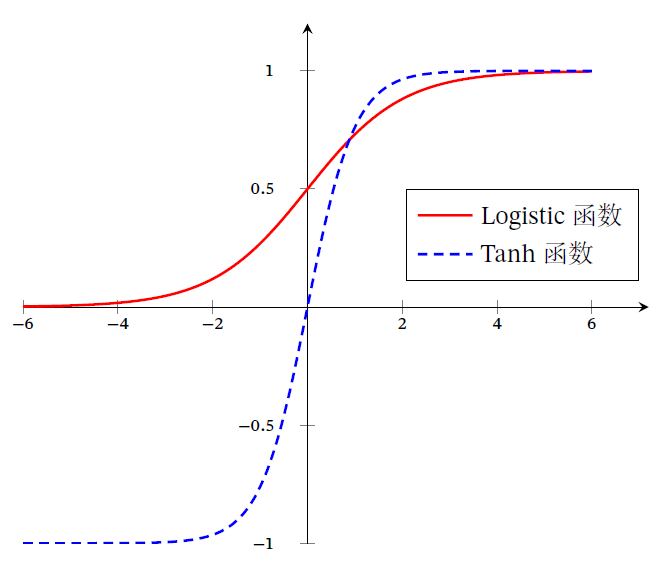
\includegraphics[width=0.4\textwidth]{sigmoid_function.png}
    \caption{Logistic 函数和Tanh 函数}
\end{figure}

\textbf{优缺点}:
Tanh函数是0均值的, 解决了Sigmoid函数的非zero-centered问题, 但是它也存在梯度消失和幂运算的问题.


\subsubsection{整流线性单位函数(Rectified Linear Unit,  ReLU)}
ReLU 实际上是一个斜坡(ramp)函数, 定义为
$$\mathrm{ReLU}(x)=
\left\{ 
\begin{array}{c}    x \\    0  \\   \end{array}
\right. =\max(0, x)
$$
\begin{figure}[!ht]
    \centering
    \includegraphics[width=\textwidth]{ReLU}
    \caption{ReLU激活函数}
\end{figure}
\paragraph{求导}
$$\frac{\rho\sigma(x)}{\rho(x)}=1-\sigma^2(x)$$

\textbf{优点}:
\begin{enumerate}
    \renewcommand{\labelenumi}{(\theenumi)}
    \item   ReLu的收敛速度比 sigmoid 和 tanh 快(梯度不会饱和, 解决了梯度消失问题);
     \item  计算复杂度低, 不需要进行指数运算;
     \item 适合用于后向传播.
\end{enumerate}

\textbf{缺点}:
\begin{enumerate} 
    \renewcommand{\labelenumi}{(\theenumi)}
\item  ReLU的输出不是zero-centered; 
\item  Dead ReLU Problem(神经元坏死现象):某些神经元可能永远不会被激活, 导致相应参数永远不会被更新(在负数部分, 梯度为0).

\textbf{产生原因}:
\begin{itemize}
    \item 参数初始化问题
    \item 学习率太高导致在训练过程中参数更新太大
\end{itemize}
 \textbf{解决方法}:采用Xavier初始化方法, 以及避免将学习率设置太大或使用adagrad等自动调节学习率的算法.
\item ReLU不会对数据做幅度压缩, 所以数据的幅度会随着模型层数的增加不断扩张.
\end{enumerate}
\paragraph{Leakly  ReLU函数}
用来解决ReLU带来的神经元坏死的问题, 可以将0.01设置成一个变量a, 其中a由后向传播学出来.但是其表现并不一定比ReLU好.

\begin{align*}
\mathrm{ELU}(x)=&
\left\{ 
\begin{array}{c c}    
    x  \ & \text{if} \  x>0 \\    
    \gamma_i x \ & \text{if} \ x \leqslant 0  \\   
\end{array} 
\right. \\
=& \max(0, x)+\gamma_i \min(0, x)
\end{align*}
其中$\gamma_i$为$x \leqslant 0 $时函数的斜率

\paragraph{ELU函数(指数线性函数)}
ELU有ReLU的所有优点, 并且解决了 Dead ReLU问题, 输出的均值接近0(zero-centered).但是计算量大, 其表现并不一定比ReLU好.
\begin{align*}
    \mathrm{ELU}(x)= &
    \left\{ 
    \begin{array}{c c}    
        x  \ & \text{if} \  x>0 \\    
        \gamma(\exp(x)-1) \ & \text{if} \ x \leqslant 0  \\   
    \end{array} 
    \right. \\
    = & \max(0, x)+\gamma_i \min(0, \gamma(\exp(x))-1)
    \end{align*}
      

\subsubsection{Entropy熵}
在信息论中, 熵用来衡量一个随机事件的不确定性.
 自信息(Self Information)表示一个随 机事件所包含的信息量. 一个随机事件发生的概率越高, 其自信息越低.如果-一个事件必然发生, 其自信息为0.
 对于一一个随机变量X (取值集合为X , 概率分布为$p(x,  x \in \mathcal{X})$, 当X=x
 时的自信息$I(x)$定义为
 \begin{equation}
      I(x)=- \log p(x).
 \end{equation} 
 
 在自信息的定义中, 对数的底可以使用2、自然常数$e$或是10.当底为2时, 自信息的单位为bit;当底为e时, 自信息的单位为nat.
 对于分布为$p(x)$的随机变量X , 其自信息的数学期望, 即熵$H(X)$定义为
 
 \begin{equation}
    \begin{split}
 H(X) &= \mathbb{E}_x\left[  I(x)\right] \\
 &= \mathbb{E}_x \left[  -\log p(x) \right] \\
 &=\sum_{x \in \mathcal{X}}p(x) \log p(x)    
\end{split}
 \end{equation}
 其中$ 0 \log 0= 0 $.
 熵越高, 则随机变量的信息越多;熵越低, 则随机变量的信息越少

\subsubsection{Cross Entropy交叉熵}
对于分布为$p(x)$的随机变量, 熵$H(p)$表示其最优编码长度.交叉熵(Cross Entropy)是按照概率分布$q$的最优编码对真实分布为$p$的信息进行编码的长度, 定义为 
\begin{equation}
 \begin{split}
        H(p, q)&= \mathbb{E}_p \left[ -\log q(x) \right]  \\
        &= - \sum_x p(x) \log q(x) 
 \end{split}
\end{equation}
 
在给定$p$的情况下, 如果$q$ 和$p$ 越接近, 交叉熵越小;如果$q$ 和$p$ 越远, 交叉熵就越大.


\subsection{神经网络}
“神经网络是由具有适应性的简单单元组成的广泛并行互连的网络, 它的组织能够模拟生物神经系统对真实世界物体所作出的交互反应”[Kohonen,  1988].

神经网络中最基本的单元是神经元模型(neuron), 最简单的神经元模型是“M-P神经元模型”.
树突对应于输入部分, 每个神经元收到n个其他神经元传递过来的输入信号, 这些信号通过带权重的连接传递给细胞体.
细胞体分为两部分, 前一部分计算总输入值(即输入信号的加权和), 后一部分先计算总输入值与该神经元阈值的差值, 然后通过激活函数的处理, 产生输出从轴突传送给其它神经元.
\begin{figure}
    \centering
    \label{MP_Model}
    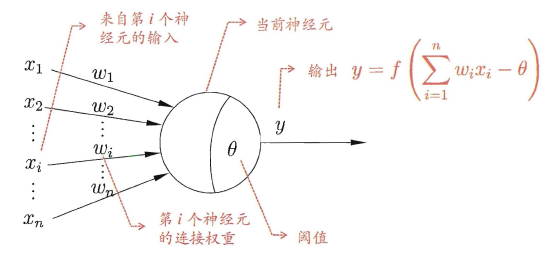
\includegraphics[width=0.9\textwidth]{MP_Modle.png}
    \caption{M-P神经元模型}
\end{figure}

神经元模型最理想的激活函数也是阶跃函数, 但阶跃函数不连续, 常采用Sigmoid函数来近似.

\subsubsection{感知器}
感知机(Perceptron)是由两层神经元组成的一个简单模型, 但只有输出层是M-P神经元, 即只有输出层神经元进行激活函数处理, 也称为功能神经元;输入层只是接受外界信号(样本属性)并传递给输出层(输入层的神经元个数等于样本的属性数目), 而没有激活函数感知机的输出层应该可以有多个神经元, 从而可以实现多分类问题, 同时两个模型所用的参数估计方法十分不同.

\begin{figure}
    \centering
    \label{MP}
    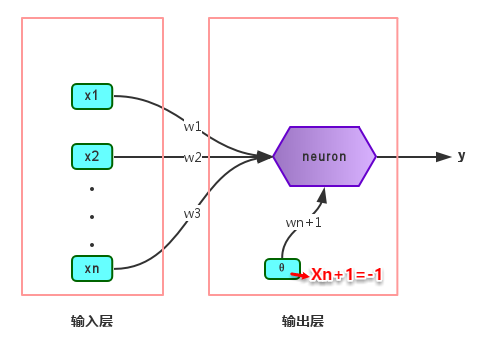
\includegraphics[width=0.5\textwidth]{simple_perceptron.png}
    \caption{简单感知机}
\end{figure}
\newpage
\paragraph{感知机学习算法} 给定个样本的训练集${(x^{(n)}, y^{(n)}}^N_{n1}$, 其中$y(n)\in {+1, -1}$, 感知器学习算法试图找到一组参数$\mathbf{w}^{\star}$, 使得对于每个样本$(x^{(n)}, y^{(n)}$有
\begin{equation}
    y^{(n)} \mathbf{w}^{\star \mathrm{T} }  \mathcal{x}^{(n)}> 0,  \forall n \in \{ 1, ..., N \}
\end{equation}
\begin{figure}
    \centering
    \label{algorithm_perceptron}
    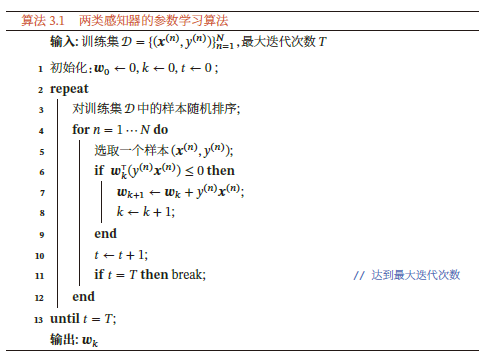
\includegraphics[width=0.9\textwidth]{algorithm_perceptron.png}
    \caption{两类感知机学习算法 }
\end{figure}

\paragraph{感知器的收敛性} 
 感知器收敛性:给定训练集 $D = {x(), y(0)}$令R是训练集
中最大的特征向量的模, 即$$R = \max_n \|x^{(n)}\|$$
如果训练集D线性可分, 两类感知器的参数学习算法3.1的权重更新次数不
超过$\frac{R^2}{\gamma^2}$次.

\paragraph{几种常见的线性模型对比} 
\begin{figure}
    \centering
    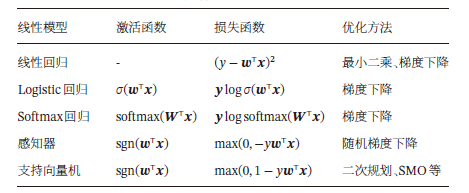
\includegraphics[width=0.7\textwidth]{linear_model.png}
    
\end{figure}
\newpage
\paragraph{不同损失函数的比较}
\begin{figure}
    \centering
    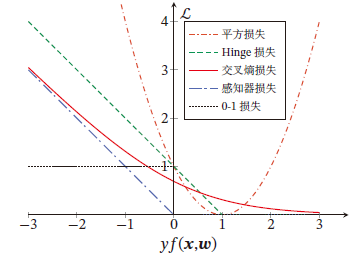
\includegraphics[width=0.7\textwidth]{loss_function.png}
    \caption{不同损失函数的比较}
\end{figure} 
一个好的损失函数应该随着$yf(\mathbf{x;w})$的增大而减少.

\subsubsection{分类问题总结}
分类问题中的决策函数需要输出离散值或是标签的后验概率.线性分类模型一般是一
个广义线性函数, 即一个或多个线性判别函数加上一个非线性激活函数.在Logistic 回归和Softmax 回归中, y 为类别的one-hot 向量表示;在感知器和支持向量机中, y 为$\{+1, -1\}$.



\subsubsection{数据集}
如果已经有了一个比较大的标注数据集, 想要完成一个有监督模型的测试, 那么通常使用均匀随机抽样的方式, 将数据集划分为训练集、验证集、测试集, 这三个集合不能有交集, 常见的比例是8:1:1。三个集合都是同分布的。
训练集就是用来训练参数的。而验证集基本是在每次epoch完成后, 测试当前模型的准确率。
对于一个模型来说, 其参数可以分为普通参数和超参数。 除强化学习外, 普通参数是可以被训练所更新。超参数不在梯度下降的更新范围内, 需要人工根据验证集调节.所以在广义上, 验证集参与了人工调参的过程, 需要一个没有经过的训练的集合, 就是测试集来测试最终准确率. \citep{training_validation_test_Su}


\subsection{前馈神经网络}
在前馈神经网络中, 不同的神经元属于不同的层, 每一层的神经元可以接受到前一层的神经元信号, 并产生信号输出到下一层.第0层叫做输入层, 最后一层叫做输出层, 中间的叫做隐藏层, 整个网络中无反馈, 信号从输入层到输出层单向传播, 可用一个有用无环图表示.

前馈神经网络也成为多层感知器(Mutlti-Layer Perceptron, MLP).但是这种叫法并不准确, 因为前馈神经网络其实是由多层Logistic回归模型(连续的非线性模型)组成, 而不是有多层感知器模型(非连续的非线性模型)组成.

下图为简单的前馈神经网络图:

\begin{figure}[!ht]
    \centering
    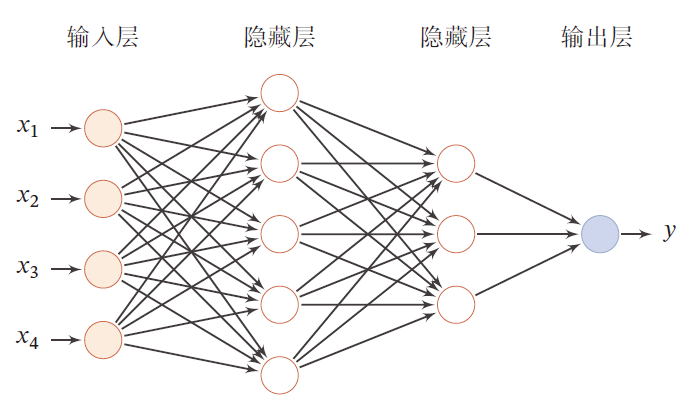
\includegraphics[width=0.6\textwidth]{FNN}
    \caption{前馈神经网络图}
\end{figure} 


神经网络中涉及的多个记号:
\begin{table}[!ht]
    \renewcommand{\arraystretch}{1.35}  
    \centering
    \begin{tabular}{cc}
        \toprule
        记号 & 含义 \\
        \midrule
        $L$ &表示神经网络的层数\\
$m^{(l)}$&表示第$ l$ 层神经元个数\\
$f_l ( \cdot ) $&表示第$ l $层神经元的激活函数\\
$W^{(l)}$   &表示第$ l-1$ 层到第 l 层的权重矩阵\\
$b^{(l)}$   &表示第$ l-1$ 层到第 l 层的偏置\\
$z^{(l)}$   &表示第 $l$ 层神经元的净输入(净活性值)\\
$a^{(l)}$   &表示第$l$层的神经元输出(活性值)\\
        \bottomrule
    \end{tabular}
\label{tabel:NerualNetwork_mark}
\caption{神经网络中涉及的记号}
\end{table}

神经网络的信息传播公式如下 
\begin{gather*}
 z^{(l)} = W^{(l)}   a^{(l-1)} + b^{(l)}\\
 a^{(l)} = f_l(z^{(l)})
\end{gather*} 
 可以合并写为 :
$$z^{(l)}=W^{(l)} f_{(l-1)} (z^{(l-1)})+b^{^{(l)}}  $$
或者 
$$a^{(l)} = f_l(W^{(l)} a^{(l-1)} + b^{(l)})$$
这样神经网络可以通过逐层的信息传递, 得到网络最后的输出$a^{(l)}$.整个网络可以看做一个符合函数$$\phi (x; W, b)$$
将向量x作为第一层的输入$a^0$, 将第 l 层的输入$a^0$,  将第L层的输出$a^{(l)}$ 作为整个函数的输出.
$$ x = a^0 \rightarrow z^1 \rightarrow a^1 \rightarrow z^2 .... \rightarrow a^{L-1} \rightarrow z^{(l)} \rightarrow a^{(l)} = \phi (x;W, b)$$
其中W,  b表示网络中所有层的连接权重和偏置. 
\paragraph{参数学习}
如果采用交叉熵损失函数, 对于样本$(x, y)$, 其损失函数为:
$$L(y, \hat{y}) = -y^T log (\hat{y})$$, 
其中 y 属于${0, 1}^T$为标签y对应的one-hot向量.

给定训练集$D={(x^{(n)}, y^{(n)},  N>=n>=0}$, 将每个样本$x^n$ 输入给前馈神经网络, 得到网络输出为$y^n$, 其在数据集$\mathcal{D}$上的结构化风险函数为:
$$R(W, b)=\frac{1}{N}\sum_{n=1}^{N} L(y^n, \hat{y}^n) + \frac{1}{2}\lambda \left \| W \right \|_F^2$$
 
其中W和b分别表示网络中所有的权重矩阵和偏置向量,  $\|W\|_F^2$ 是正则化项, 用来防止过拟合, $\lambda$是为正数的超参数, $\lambda$越大, W越接近于0.这里的$(\|W\|_F)^2$一般使用Frobenius范数.
 
有了学习准则和训练样本, 网络参数可以通过梯度下降法来进行学习.在梯度下降方法的每次迭代过程中, 第l层的参数$ W^{(l)} $和$ b^{(l)}$ 参数更新方式为:
\begin{gather*}
    W^{(l)} \leftarrow W^{(l)} - \alpha \frac{\partial R(W, b)}{\partial W^{(l)}}=W^{(l)} - \alpha ( \frac{1}{N} \sum_{n=1}^{N}(\frac{\partial L(y^n, \hat{y}^n)}{\partial W^{(l)}}) + \lambda W^{(l)} )\\b^{(l)} \leftarrow b^{(l)} - \alpha \frac{\partial R(W, b)}{\partial b^{(l)}}=b^{(l)} - \alpha ( \frac{1}{N} \sum_{n=1}^{N}(\frac{\partial L(y^n, \hat{y}^n)}{\partial b^{(l)}}) ) 
\end{gather*}
其中$\alpha$为学习率.
梯度下降法需要计算损失函数对参数的偏导数, 如果通过链式法则逐一对每个参数进行求偏导效率比较低.在神经网络的训练中经常使用反向传播算法来高效的计算梯度. 
\subsubsection{反向传播算法}
基于误差的反向传播算法(backpropagation, BP)的前馈神经网络训练过程可以分为以下三步:
\begin{enumerate} 
    \renewcommand{\labelenumi}{(\theenumi)}
\item 前馈计算每一层的净输入$z^{(l)}$ 和激活值 $a^{(l)}$, 直到最后一层
\item 反向传播计算每一层的误差项
\item 计算每一层参数的偏导数, 并更新参数
\end{enumerate}

它利用均方误差和梯度下降的方法来实现对网络连接权值的修改.网络连接权值的修改是为了使误差平方和最小.该算法首先对网络的连接值赋一个小的值, 然后选择一个训练样本来计算相对于这个样本的误差梯度.
\begin{figure}
    \centering
    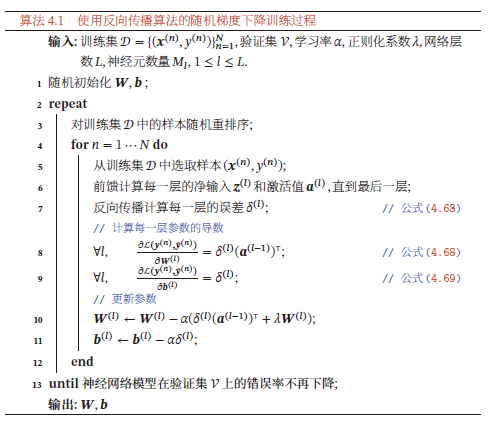
\includegraphics[width=0.7\textwidth]{algorithm_bp.png}
\end{figure} 

\subsubsection{优化问题}
\paragraph{非凸优化问题}
使用非凸的损失函数
如平方误差损失函数和交叉熵损失函数
\paragraph{梯度消失问题}
由于Sigmoid 型函数的饱和性, 饱和区的导数更是接近于0.这样, 误差经
过每一层传递都会不断衰减.当网络层数很深时, 梯度就会不停衰减, 甚至消
失, 使得整个网络很难训练.这就是所谓的梯度消失问题(Vanishing Gradient
Problem), 也称为梯度弥散问题.

\subsubsection{通用近似定理}
通用近似定理( Universal Approximation Theorem) 

令$\Phi(\cdot)$是一个非常数、有界、单调递增的连续函数,  $\mathcal{J}_D$是一个D维的单位超立方体$[0, 1]^D$,  $C(\mathcal{p})$是定义在$\mathcal{J}_D$.上的连续函数集合对于任何-一个函数$f \in C(\mathcal{J}_D)$, 存在一个整数M, 和一组实数$v_m, b_m \in R$以及实数向量$v_m \in R^D, m= 1,  \cdots,  M$ 以至于我们可以定义函数
$$F(x) =2v_m \phi(v_m^T x + b_m)$$
作为函数f的近似实现, 即
$$|F(x)- f(x)|< \upsilon_i \forall x \in (\mathcal{J}_D) $$
其中$ \upsilon > 0$是一个很小的正数.


一个前馈神经网络如果具有线性输出层和至少一层具有任何一种"挤压"性质的激活函数(例如 sigmoid激活函数)的隐藏层, 只要给予网络足够数量的隐藏单元, 它可以以任意的精度来近似任何一个任何定义在实数空间$ R^D$中的有界闭集函数(Borel 函数). 神经网络的通用近似性质也被证明对于其他类型的激活函数, 比如ReLU, 也都是适用的.

学习失败原因:
\begin{itemize}
    \item 用于训练的优化算法可能找不到用于期望函数的参数值.
    \item 训练算法可能由于过拟合而选择了错误的函数.
\end{itemize}
\subsection{循环神经网络}

\textbf{前馈网络的一些不足}
\begin{itemize}
    \item 连接存在层与层之间, 每层的节点之间是无连接的(无循环)
    \item 输入和输出的维数都是固定的, 不能任意改变.无法处理变长的序列数据.
    \item 假设每次输入都是独立的, 也就是说每次网络的输出只依赖于当前的输入.
\end{itemize}

\textbf{循环神经网络}(Recurrent Neural Network, RNN)通过使用带自反馈的神经元, 能够处理任意长度的序列, 比前馈神经网络更加符合生物神经网络的结构.
给定-一个输入序列$x_{1:T} =(x_1, x_2,  .... x_t, .... x_T)$, 循环神经网络通过下面公式更新带反馈边的隐藏层的活性值$h_t$:
$$h_t= f(h_t-1, x_t)$$
其中$h_0= 0, f( \cdot )$为一个非线性函数, 可以是一个前馈网络.
\begin{figure}[!htb]
    \center
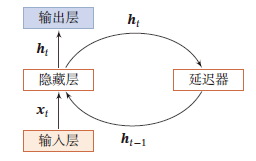
\includegraphics[width=0.9\textwidth]{RNN_sample.png}
\caption{循环神经网络}
\end{figure}


图中“延时器”为一个虚拟单元, 记录神经元的最近一次(或几次)活性值.
\subsubsection{简单循环网络}
Simple Recurrent Network, SRN \citep{elman1990finding} 
 
$$h_t = f(Uh_t-1 +Wx_t + b)$$
\begin{figure}[!htb]
    \center
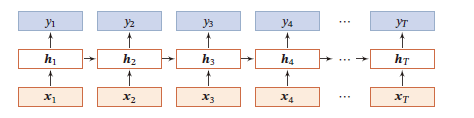
\includegraphics[width=0.7\textwidth]{simple_RNN.png}
\caption{按时间展开的循环神经网络}
\end{figure}


\subsubsection{循环神经网络的计算能力}
循环神经网络的拟合能力十分强大.一个完全连接的循环网络是任何非线性动力系统的近似器.
如果一个完全连接的循环神经网络有足够数量的sigmoid 型隐藏神经元, 它可以以任意的准确率去近似任何一个非线性动力系统

\begin{equation*}
    \begin{split}
        S_t &= g(S_{t-1}, x_t) \\
        y_i & = o(s_t)
    \end{split}
\end{equation*}
其中$S_t$为每个时刻的隐状态, $x_t$是外部输入, $g(\cdot)$是可测的状态转换函数, 
$o(\cdot)$ 是连续输出函数, 并且对状态空间的紧致性没有限制.
 
\begin{figure}[!htb]
    \center
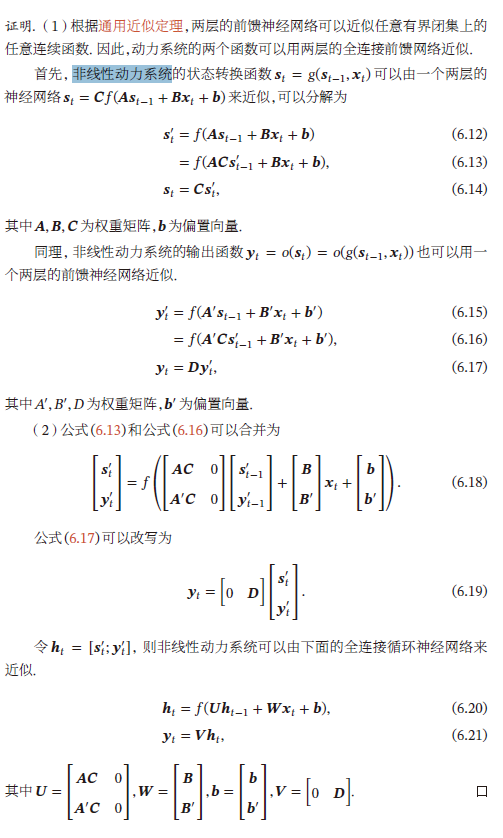
\includegraphics[width=0.8\textwidth]{RNN_univesal.png}
\end{figure}



% \subsubsection{循环神经网络在机器学习中的应用}


 \paragraph{长期依赖(Long-Term Dependencies)问题}
如果相关信息和当前预测位置之间的间隔就相当的大, 在这个间隔不断增大时,  RNN会难以学习到连接如此远的信息。(梯度消失和梯度爆炸)

在序列中, 依赖现象较为明显, 如主谓依赖、名词与动词单复数的依赖。在较短范围内, 这种依赖能够被传统的语言模型(如n-gram, 神经语言模型)刻画, 但是长距离依赖则是传统语言模型难以刻画的。长距离依赖是序列建模的重要刻画内容之一.
循环神经网络在进行梯度反向传播时也面临着梯度消失和梯度爆炸问题, 只是表现在时间轴上, 即如果输入序列很长,  梯度难以更新。



解决: LSTM GRU Attention


\paragraph{序列到类别模式}

输入为序列, 输出为类别.比如在文本分类中, 输入数据为单词的序列, 输出为该文本的类别.

假设一个样本$$ x_{1:T}=(x_1, ...,  x_T)$$ 为一个长度为T的序列, 输出为一个类别 $y \in {1,  2,  \dot C}$.可以将样本x按不同时刻输入到RNN中, 得到不同时刻的隐藏状态 $h_1,  \dots,  h_T$ .可以将 $h_T$看作整个序列的最终表示, 并输入给分类器 $g(\cdot)$进行分类,  $\hat{y}=g(h_T)$

其中 $g(\cdot)$可以是简单的线性分类器如Logistic回归, 或复杂分类器如前馈神经网络.

除了将最后时刻的状态作为小于列表示之外, 还可以对整个序列的所有状态进行平均, 用这个平均状态作为整个序列的表示:
\begin{figure}[!htb]
    \center
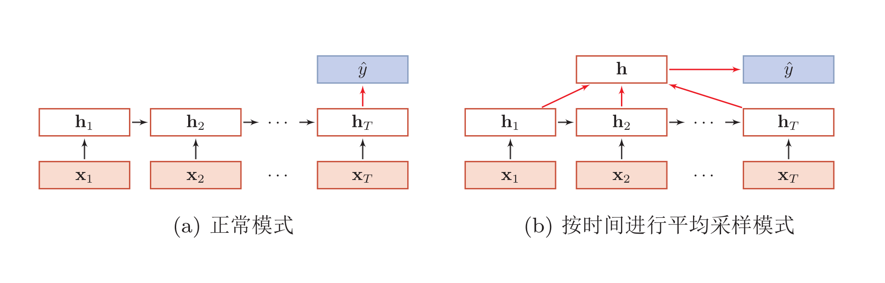
\includegraphics[width=0.8\textwidth]{RNN_model1.png}
\caption{序列到类别模式}
\end{figure}


\paragraph{同步的序列到序列模式}

\begin{figure}[!htb]
    \center
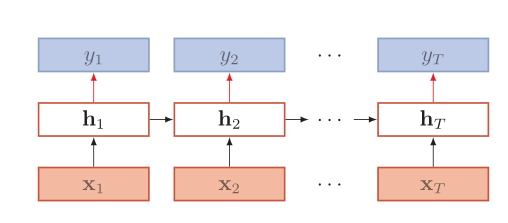
\includegraphics[width=0.8\textwidth]{RNN_model2.png}
\caption{同步的序列到序列模式}
\end{figure}
每一时刻都有输入和输出, 输入序列和输出序列的长度相同, 如词性标注(Part-of-Speech Tagging)中, 每一个单词都需要标注其对应的词性标签.

输入为一个长度为T的序列$$ x_{1:T}=(x_1, ...,  x_T)$$, 输出为序列$y_{1:T}=(y_1, ...,  y_T)$.样本x按不同时刻输入到RNN中, 并得到不同时刻的隐状态$h_1,  \dots,  h_T$ .每个时刻的隐状态$h_t$代表了当前时刻和历史的信息, 并输入给分类器 $g(\cdot)$得到当前时刻的标签 $ \hat{y}_t$ .
$$\hat{y}= g(h_t),  \  \forall t \in [1, T]$$



\paragraph{异步的序列到序列模式}
也称为编码器-解码器(Encoder-Decoder)模型, 输入序列和输出序列不需要严格的对应关系, 也不需要保持相同的长度.类似于机器翻译.

输入为一个长度为T的序列 $ x_{1:T}=(x_1, ...,  x_T)$, 输出长度为M的序列 $ y_{1:T}=(y_1, ...,  y_T)$ .先将样本x按不同时刻输入到RNN中(编码器), 得到其编码 $h_T$ , 然后使用另一个RNN(解码器), 得到输出序列$ \hat{y}_{1:m}$ , 为了建立输出序列之间的依赖关系, 在解码器中通常使用非线性的自回归模型.

\begin{equation}
    \begin{split}
        h_t &= f_1(hp_1, x),   \forall t \in [1, T] \\
    h_{T+t}& = f_2(h_{T+t-1}, \hat{y}_{t-1}),  \forall t\in[1, M]\\
    \hat{y}&= g(h_{T+t}),   \forall t\in[1, M]
    \end{split} 
\end{equation}

其中 $f(\cdot)$ 为编码器和解码器的神经网络,  $g(\cdot)$ 为分类器,  $\hat{Y}_t$为预测输出 $\hat{y}_t$的向量表示.
\begin{figure}[!htb]
    \center
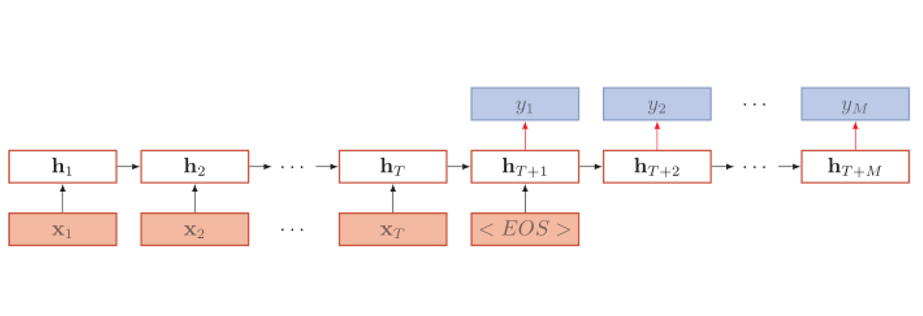
\includegraphics[width=0.8\textwidth]{RNN_model3.png}
\caption{异步的序列到序列模式}
\end{figure}

% \subsubsection{========}

% 将字符打乱顺序普通神经网络无法预测下一个

% \begin{tikzcd}
%     &  \arrow[rd,  "\mathbf{b}^{(l)} \to \mathbf{I}_{m^{(l)}}"] &                                      &                                         & {\partial{L}(\mathbf{y},  \hat{\mathbf{y}})} \arrow[lld,  "\delta^{l}"'] \arrow[d,  "\delta^{l+1}"] &  \\
% \mathbf{a}^{(l-1)} \arrow[rr,  "W_{ij}^{(l)} \to a_{j}^{(l-1)}"'] &                                                          & \sum \mathbf{z}^{(l)} \arrow[r,  "f"] & \mathbf{a}^{(l)} \arrow[r,  "W^{(l+1)}"] & \mathbf{z}^{(l+1)} \arrow[r,  "f"]                                                                &  \\
%     &  \arrow[ru]                                              &                                      &                                         &                                                                             & 
% \end{tikzcd}


% \textbf{RNN应用在知识图谱--图网络}

\subsubsection{简介实现}

\begin{enumerate}
    \item  使用困惑度评价模型。
    \item  在迭代模型参数前裁剪梯度。
    \item  对时序数据采用不同采样方法将导致隐藏状态初始化的不同
\end{enumerate}

\subsection{通过时间反向传播}
BPTT 算法将循环神经网络看作一个展开的多层前馈网络, 其中“每一层”对应循环网络中的“每个时刻”, 所有层的参数是共享的, 因此参数的真实梯度是所有“展开层”的参数梯度之和.
% \begin{figure}[!htb]
%     \center
% 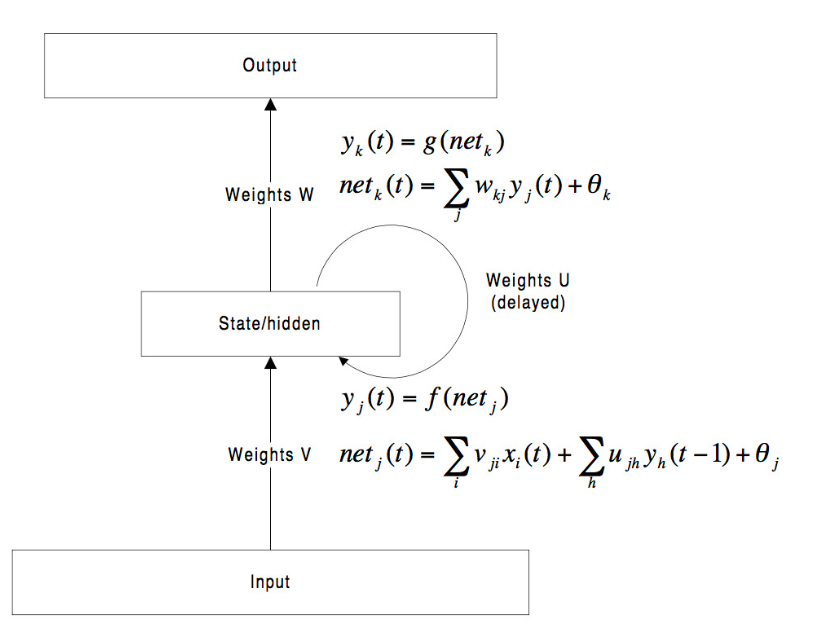
\includegraphics[width=0.6\textwidth]{BPTT.png}
% \caption{BPTT算法}
% \end{figure}
假设
\begin{itemize}
\item 激活函数$\Phi(x)=x$, 
\item t时刻输入$\boldsymbol{x}_t \in \mathbb{R}^d$, 
\item 标签 $y_t$
\item 隐藏状态 $\boldsymbol{h}_t \in \mathbb{R}^h$
\item 隐藏层权重 
$$\boldsymbol{W}_{hx} \in \mathbb{R}^{h \times d}$$
$$\boldsymbol{W}_{hh} \in \mathbb{R}^{h \times h}$$
\item 输出层权重
$\boldsymbol{W}_{qh} \in \mathbb{R}^{q \times h}$
\item
t时刻输出$\boldsymbol{o}_t \in \mathbb{R}^q$, 

$$\boldsymbol{o}_t = \boldsymbol{W}_{qh} \boldsymbol{h}_{t}.$$
\item 
t 时刻损失 $\ell(\boldsymbol{o}_t,  y_t)$
时间步数为T的损失函数$$L = \frac{1}{T} \sum_{t=1}^T \ell (\boldsymbol{o}_t,  y_t).$$
\end{itemize}
  
prod运算符将根据两个输⼊矩阵的形状, 在必要的操作(如转置和互换输⼊位置)后对两个输⼊做乘法。


计算
目标函数有关各时间步输出层变量的梯度 $\partial L/\partial \boldsymbol{o}_t \in \mathbb{R}^q$
$$\frac{\partial L}{\partial \boldsymbol{o}_t} =  \frac{\partial \ell (\boldsymbol{o}_t,  y_t)}{T \cdot \partial \boldsymbol{o}_t}.$$

有关模型参数$\boldsymbol{W}_{qh}$的梯度
$$
\frac{\partial L}{\partial \boldsymbol{W}_{qh}} 
= \sum_{t=1}^T \text{prod}\left(\frac{\partial L}{\partial \boldsymbol{o}_t},  \frac{\partial \boldsymbol{o}_t}{\partial \boldsymbol{W}_{qh}}\right) 
= \sum_{t=1}^T \frac{\partial L}{\partial \boldsymbol{o}_t} \boldsymbol{h}_t^\top.
$$
 
有关最终时间步隐藏状态的梯度$\partial L/\partial \boldsymbol{h}_T \in \mathbb{R}^h$
$$
\frac{\partial L}{\partial \boldsymbol{h}_T} = \text{prod}\left(\frac{\partial L}{\partial \boldsymbol{o}_T},  \frac{\partial \boldsymbol{o}_T}{\partial \boldsymbol{h}_T} \right) = \boldsymbol{W}_{qh}^\top \frac{\partial L}{\partial \boldsymbol{o}_T}.
$$


对于时间步$t < T$, 

目标函数有关时间步$t < T$的隐藏状态的梯度$\partial L/\partial \boldsymbol{h}_t \in \mathbb{R}^h$需要按照时间步从大到小依次计算:

$$
\frac{\partial L}{\partial \boldsymbol{h}_t}
= \text{prod}\left(\frac{\partial L}{\partial \boldsymbol{h}_{t+1}},  \frac{\partial \boldsymbol{h}_{t+1}}{\partial \boldsymbol{h}_t} \right)
+ \text{prod}\left(\frac{\partial L}{\partial \boldsymbol{o}_t},  \frac{\partial \boldsymbol{o}_t}{\partial \boldsymbol{h}_t} \right)
= \boldsymbol{W}_{hh}^\top \frac{\partial L}{\partial \boldsymbol{h}_{t+1}} + \boldsymbol{W}_{qh}^\top \frac{\partial L}{\partial \boldsymbol{o}_t}.
$$

将上面的递归公式展开, 对任意时间步$1 \leq t \leq T$, 我们可以得到目标函数有关隐藏状态梯度的通项公式
$$
\frac{\partial L}{\partial \boldsymbol{h}_t} 
= \sum_{i=t}^T {\left(\boldsymbol{W}_{hh}^\top\right)}^{T-i} \boldsymbol{W}_{qh}^\top \frac{\partial L}{\partial \boldsymbol{o}_{T+t-i}}.
$$
 
隐藏层中模型参数的梯度$\partial L / \partial \boldsymbol{W}_{hx} \in \mathbb{R}^{h \times d}$和$\partial L / \partial \boldsymbol{W}_{hh} \in \mathbb{R}^{h \times h}$。
$$
\begin{aligned}
\frac{\partial L}{\partial \boldsymbol{W}_{hx}} 
&= \sum_{t=1}^T \text{prod}\left(\frac{\partial L}{\partial \boldsymbol{h}_t},  \frac{\partial \boldsymbol{h}_t}{\partial \boldsymbol{W}_{hx}}\right) 
= \sum_{t=1}^T \frac{\partial L}{\partial \boldsymbol{h}_t} \boldsymbol{x}_t^\top, \\
\frac{\partial L}{\partial \boldsymbol{W}_{hh}} 
&= \sum_{t=1}^T \text{prod}\left(\frac{\partial L}{\partial \boldsymbol{h}_t},  \frac{\partial \boldsymbol{h}_t}{\partial \boldsymbol{W}_{hh}}\right) 
= \sum_{t=1}^T \frac{\partial L}{\partial \boldsymbol{h}_t} \boldsymbol{h}_{t-1}^\top.
\end{aligned}
$$



%  \textbf{偏置项}
\subsection{语言模型}

标准定义:对于语言序列 $w_1, w_2, \dots,  w_n$, 语言模型就是计算该序列的概率, 即 $P(w_1, w_2,  \dots,  w_n)$ .
从机器学习的角度来看:语言模型是对语句的概率分布的建模.
通俗解释:判断一个语言序列是否是正常语句, 即人是否可理解, 例如 $P(I am Light) > P(Light I am)$ .
\paragraph{n元语法}

当序列长度增加时, 计算和存储多个词共同出现的概率的复杂度会呈指数级增加. n 元语法通过马尔可夫假设(虽然并不一定成立)简化了语言模型的计算.这里的马尔可夫假设是指一个词的出现只与前面 n 个词相关, 即 n 阶马尔可夫链(Markov chain of order n).如果 n=1 , 那么有 $P(w_3∣w_1, w_2)=P(w_3∣w_2)$ .如果基于 n-1 阶马尔可夫链, 我们可以将语言模型改写为
$$P(w_1, w_2, \cdots , w_T) \approx \Pi_{t=1}^T P(w_t|w_t-(n-1), \cdots, w_{t-1})$$.
以上也叫 n 元语法(n-grams). 它是基于 n-1 阶马尔可夫链的概率语言模型.当 n 分别为1、2和3时, 我们将其分别称作一元语法(unigram)、二元语法(bigram)和三元语法(trigram).

\subsection{深度循环神经网络}
含有多个隐藏层的循环神经网络, 也称作深度循环神经网络。下图演示了一个, \textbf{每个隐藏状态不断传递至当前层的下一时间步和当前时间步的下一层}。

 \begin{figure}[!htb]
    \center
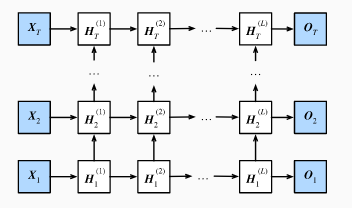
\includegraphics[width=0.6\textwidth]{deep_rnn.png}
\caption{有$L$个隐藏层的深度循环神经网络}
\end{figure}
 

具体来说, 在时间步$t$里, 设小批量输入$\mathbf{X}_t \in \mathbb{R}^{n \times d}$(样本数为$n$, 输入个数为$d$), 第$l$隐藏层($l=1, \ldots, L$)的隐藏状态为$\mathbf{H}_t^{(l)}  \in \mathbb{R}^{n \times h}$(隐藏单元个数为$h$), 输出层变量为$\mathbf{O}_t \in \mathbb{R}^{n \times q}$(输出个数为$q$), 且隐藏层的激活函数为$\phi$。第1隐藏层的隐藏状态和之前的计算一样:
$$\mathbf{H}_t^{(1)} = \phi(\mathbf{X}_t \mathbf{W}_{xh}^{(1)} + \mathbf{H}_{t-1}^{(1)} \mathbf{W}_{hh}^{(1)}  + \mathbf{b}_h^{(1)}), $$
其中权重$\mathbf{W}_{xh}^{(1)} \in \mathbb{R}^{d \times h}$、$\mathbf{W}_{hh}^{(1)} \in \mathbb{R}^{h \times h}$和偏差 $\mathbf{b}_h^{(1)} \in \mathbb{R}^{1 \times h}$分别为第1隐藏层的模型参数。

当$1 < l \leq L$时, 第$l$隐藏层的隐藏状态的表达式为
$$\mathbf{H}_t^{(l)} = \phi(\mathbf{H}_t^{(l-1)} \mathbf{W}_{xh}^{(l)} + \mathbf{H}_{t-1}^{(l)} \mathbf{W}_{hh}^{(l)}  + \mathbf{b}_h^{(l)}), $$
其中权重$\mathbf{W}_{xh}^{(l)} \in \mathbb{R}^{h \times h}$、$\mathbf{W}_{hh}^{(l)} \in \mathbb{R}^{h \times h}$和偏差 $\mathbf{b}_h^{(l)} \in \mathbb{R}^{1 \times h}$分别为第$l$隐藏层的模型参数。
最终, 输出层的输出只需基于第$L$隐藏层的隐藏状态:
$$\mathbf{O}_t = \mathbf{H}_t^{(L)} \mathbf{W}_{hq} + \mathbf{b}_q, $$
其中权重$\mathbf{W}_{hq} \in \mathbb{R}^{h \times q}$和偏差$\mathbf{b}_q \in \mathbb{R}^{1 \times q}$为输出层的模型参数。

\subsubsection{LSTM}
Long short time memory(LSTM),  由Hochreiter 和Schmidhuber提出。\citep{HochreiterLong}。
LSTM传递两部分信息状态信息$h_{t-1}$, 记忆信息$c_{t-1}$.两者相互作用。LSTM通过门单元来动态地选择遗忘多少以前的信息和记忆多少当前的信息。包括遗忘门, 输入门和输出门。
$x_t$ 表示时刻t 的输入向量, $h_{t−1}$ 是时刻t−1 的循环单元的输出, 
\begin{figure}[!htb]
    \center
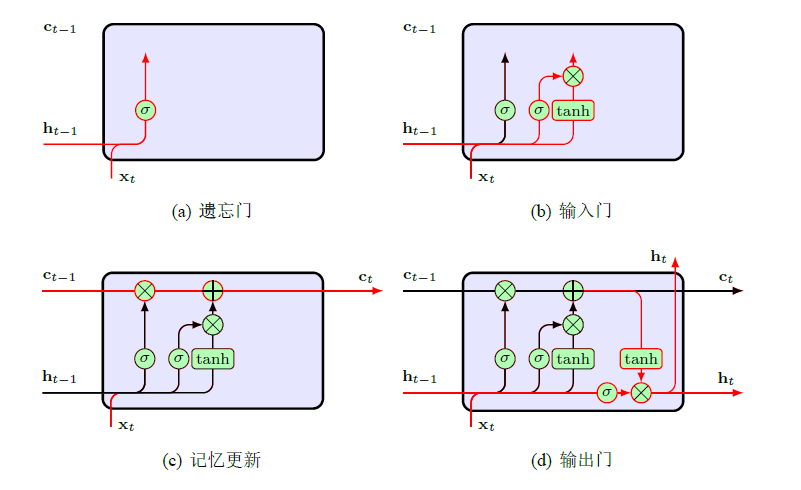
\includegraphics[width=0.9\textwidth]{LSTM.png}
\caption{LSTM 中的门控结构}
\end{figure}
LSTM结构的三部分:
\paragraph{遗忘} 通过遗忘门实现.
$f_t=\sigma (W_f h_{t-1, x_t}+b_f)$$ W_f $权值, $b_f$偏置, 该公式是对$[h_{t−1}, x_t]$ 进行变换, 并得到一个实数向量$f_t$。$f_t$ 的每一维都可以被理解为一个“门”, 它决定可以有多少信息被留下(或遗忘)。

\paragraph{记忆更新}
门控参数$\mathbf{i}_t$
\begin{align*}
    \mathbf{i}_t=\sigma(W[h_t-1, x_t])+b_i \\
    \hat{c}=Than(W_c[h_{t-1}, x_t]+b_i])
    \end{align*}

当前需记忆信息, 记为$\mathbf{i} \cdot \hat{c}_t$

\paragraph{输出}
\begin{align*}
\mathbf{o}_t  & =\sigma(W_o[h_{t-1, x_t]+b_o}) \\
\mathbf{h}_t & ={o}_t \cdot Than(c_t)
\end{align*}
 

\paragraph{循环神经网络和递归神经网络}

循环神经网络(Recurrent NN)是在时间维度上的展开, 代表信息在时间维度从前往后的的传递和积累, 可以类比markov, 后面的信息的概率建立在前面信息的基础上, 在神经网络结构上表现为后面的神经网络的隐藏层的输入是前面的神经网络的隐藏层的输出;有环结构.

递归神经网络(Recursive NN)是空间维度的展开, 是一个树结构, 无环结构.
用循环神经网络(Recurrent NN)来建模的话就是假设句子后面的词的信息和前面的词有关, 而用递归神经网络(Recursive NN)来建模的话, 就是假设句子是一个树状结构, 如由几个部分(主语, 谓语, 宾语)组成.

\subsubsection{LSTM实现}
使用周杰伦歌词, 训练模型并根据前缀“油画”创作⻓度为50个字符的⼀段歌词。每过40个迭代周期便根据当前训练的模型创作⼀段歌词。
\begin{figure}[!ht]
    \center
    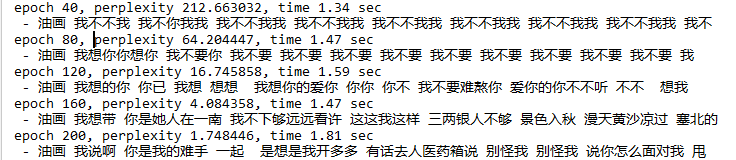
\includegraphics[width=0.8\textwidth]{lyrics.png}
    \end{figure} 
\subsubsection{GRU}
Gated Recurrent Unit (GRU) 门循环单元
\textbf{GRU 中的门控结构}

\begin{figure}[!htb]
\centering
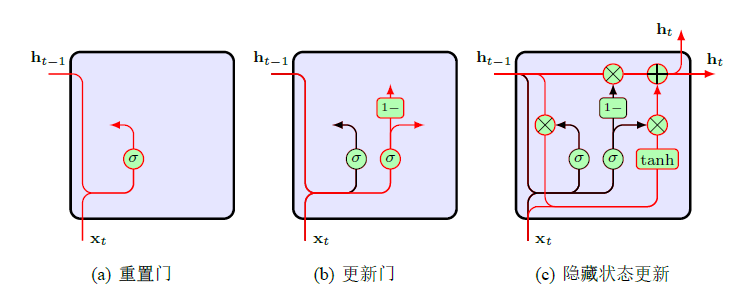
\includegraphics[width=0.9\textwidth]{GRU.png}
\caption{GRU中的门控结构}
\end{figure}

GRU对LSTM进行了简化, 把循环单元状态$h_t$和记忆$c_t$合并为状态$h_t$, 
LSTM传递的两部分信息状态信息$h_{t−1}$和记忆信息$c_{t−1}$。
GRU有两个门, 
\begin{itemize}
    \item 重置门$r_t$:用来控制前一时刻隐藏状态的记忆程度.
    \item 更新门$u_t$:更新记忆, 使用一个门同时完成遗忘和记忆两种操作, 
\end{itemize}

GRU计算流程:

step1: 更新门$r_t$和重置门$u_t$计算
\begin{align*}
\mathbf{r}_t  & =\sigma(W_r[h_{t-1, x_t]}) \\
\mathbf{u}_t &  =\sigma(W_u[h_{t-1, x_t]})
\end{align*} 

step2: 更新当前隐藏状态 
$$\hat{h}_t=Than(W_h[r_t \cdot h_{t-1}, X_t])$$

step3: 计算更新后的隐藏状态(更新记忆)
$$h_t=(1-u_t) \cdot h_{t-1} + u_t\cdot \hat{h}_t$$

\subsubsection{改进}
\paragraph{双向模型}

\begin{figure}[htp]
    \centering
    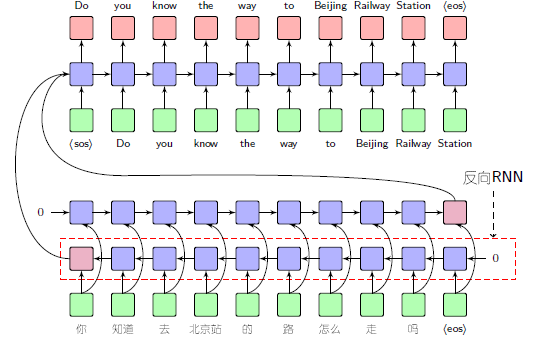
\includegraphics[width=0.9\textwidth]{dual_direction_ML.png}
    \caption{基于双向循环神经网络的机器翻译模型结构}
    \end{figure}
自左向右的模型只考虑了左侧的上下文, 因此可以用自右向左的模型对右侧上下文建模, 最终将两个模型融合同时送给编码端

\begin{figure}[htp]
    \centering
    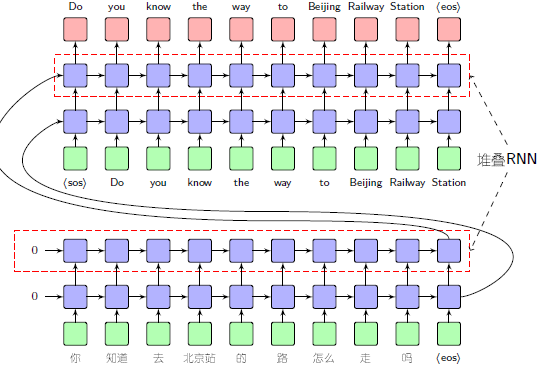
\includegraphics[width=0.9\textwidth]{multiNet_NML.png}
    \caption{基于双层循环神经网络的机器翻译模型结构}
    \end{figure}
 堆叠更多层的网络, 可以提升模型的表示能力
 
\subsection{Attention}

简单的编码器-解码器的问题:
将源语言句子编码为一个实数向量虽然很有效, 但是有明显问题
\begin{itemize}
    \item 
    整个句子编码到一个向量里可能会有信息丢失
    \item 
    缺少源语单词与目标语单词之间的对应。某种意义上讲, 一个目标语单词的生成无法区分不同源语单词的贡献
\end{itemize}
翻译是具有很强的局部性的, 有些词之间会有更紧密的关系
源语词和目标语词的对应并不是均匀的, 甚至非常稀疏, 比如, 一些短语的生成仅依赖于源文中的少数词, 这些关系可以在表示模型中考虑
\textbf{关注的"局部性"在图像处理、语音识别等领域也有广泛讨论}
\begin{figure}[htp]
    \centering
    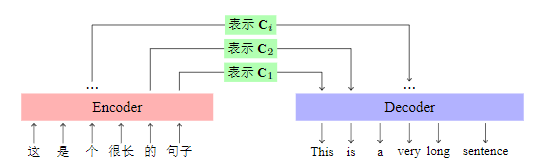
\includegraphics[width=0.9\textwidth]{attention1.png}
    \caption{使用注意力机制的翻译模型}
    \end{figure}
    \paragraph{上下文向量}
可以将注意力机制看做是一种对接收到的信息的加权处理, 上下文向量$\mathbf{C}_j$被定义为对不同时间步编码器输出的状态序列$\{ \mathbf{h}_1,  \mathbf{h}_2, ..., \mathbf{h}_m \}$进行加权求和, 如下:
    \begin{eqnarray}
    \mathbf{C}_j=\sum_{i} \alpha_{i, j} \mathbf{h}_i
    \end{eqnarray}
其中, $\alpha_{i, j}$是{\small\sffamily\bfseries{注意力权重}}\index{注意力权重}(Attention Weight)\index{Attention Weight}, 它表示目标语第$j$个位置与源语第$i$个位置之间的相关性大小。

\begin{figure}[htp]
    \centering
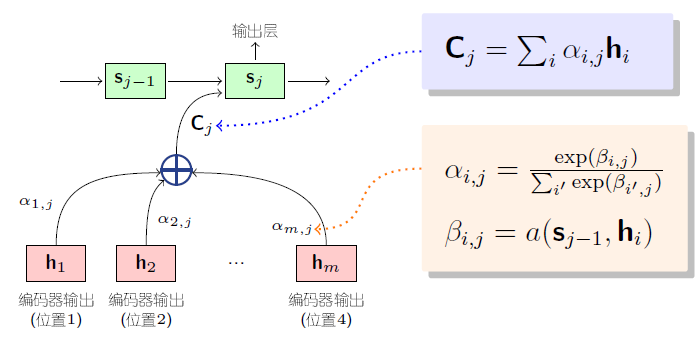
\includegraphics[width=0.9\textwidth]{context_vector_cacl.png}
    \caption{上下文向量计算过程实例}
    \end{figure}

\subsection{Transformer}
使用循环神经网络对源语、目标语建模进行信息提取效果很好, 但是当序列过长时, 词汇之间信息传递距离过长, 导致模型的信息提取能力变差。
\begin{figure}[htp]
    \centering
    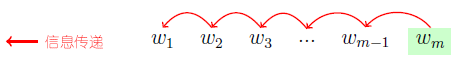
\includegraphics[width=0.9\textwidth]{self-attention1.png}
    \caption{循环神经网络中单词之间的依赖关系}
    \end{figure}
 能否将不同位置之间的词汇间信息传递的距离拉近为1? 
 \begin{figure}[htp]
    \centering
    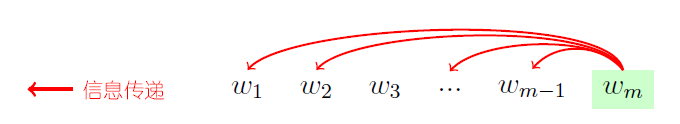
\includegraphics[width=0.9\textwidth]{self_attention2.png}
    \caption{自注意力机制中单词之间的依赖关系}
    \end{figure}


\textbf{自注意力机制(Self-Attention)}可以很好的解决长距离依赖问题, 增强信息抽取能力, 在长距离语言建模任务取得了很好的效果
 自注意力机制则是将源语言每个位置的表示$h_i$看做query, 同时将所有位置的表示看做key和value
 Transformer是Google在2017年提出的一个新型网络结构, 完全基于注意力机制, 取得了很好成绩!通过自注意机制能够直接获取全局信息, 不像RNN需要逐步进行信息提取, 也不像CNN只能获取局部信息, 可以并行化操作, 提高训练效率, Transformer不仅仅被用于神经机器翻译任务, 还广泛用于其他NLP任务、甚至图像处理任务。
 %----------------------------------------------
\begin{figure}[htp]
    \centering
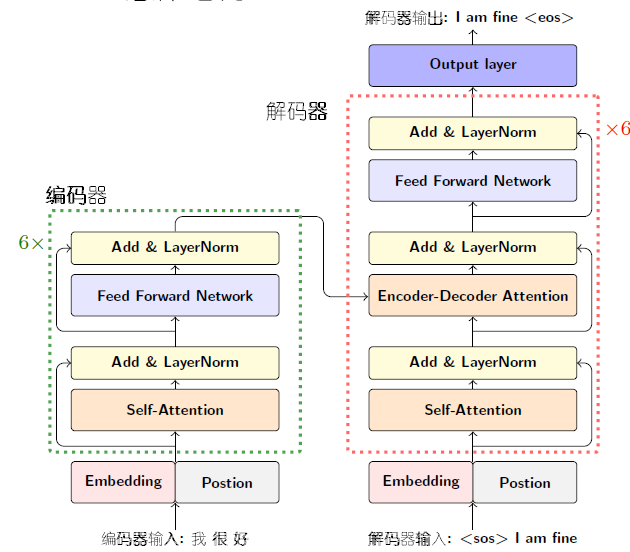
\includegraphics[width=0.9\textwidth]{Transformer1.png}
    \caption{Transformer结构}
    \label{Transformer}
    \end{figure}
    \parinterval 图\ref{Transformer} 展示了经典的Transformer结构。解码器由若干层组成(绿色虚线框就代表一层)。每一层(layer)的输入都是一个向量序列, 输出是同样大小的向量序列, 而Transformer层的作用是对输入进行进一步的抽象, 得到新的表示结果。不过这里的层并不是指单一的神经网络结构, 它里面由若干不同的模块组成, 包括:
    \begin{itemize}
        \vspace{0.5em}
        \item {\small\sffamily\bfseries{自注意力子层}}\index{自注意力子层}(Self-attention Sub-layer)\index{Self-attention Sub-layer}:使用自注意力机制对输入的序列进行新的表示;
        \vspace{0.5em}
        \item {\small\sffamily\bfseries{前馈神经网络子层}}\index{前馈神经网络子层}(Feed-forward Sub-layer)\index{Feed-forward Sub-layer}:使用全连接的前馈神经网络对输入向量序列进行进一步变换;
        \vspace{0.5em}
        \item {\small\sffamily\bfseries{残差连接}}\index{残差连接}(Residual Connection, 标记为``Add'')\index{Residual Connection}:对于自注意力子层和前馈神经网络子层, 都有一个从输入直接到输出的额外连接, 也就是一个跨子层的直连。残差连接可以使深层网络的信息传递更为有效;
        \vspace{0.5em}
        \item {\small\sffamily\bfseries{层正则化}}\index{层正则化}(Layer Normalization)\index{Layer Normalization}:自注意力子层和前馈神经网络子层进行最终输出之前, 会对输出的向量进行层正则化, 规范结果向量取值范围, 这样易于后面进一步的处理。
        \vspace{0.5em}
        \end{itemize}

\subsubsection{残差连接}
在Transformer中, 编码器、解码器分别由6层网络组成, 每层网络又包含多个子层(自注意力网络、前馈神经网络)。Transformer实际上是一个很深的网络结构, 在训练过程中容易出现梯度消失的情况在这里引入了在图像领域用来训练深层网络的技术, 残差网络来避免上述问题.
\begin{eqnarray}
    x_{l+1} = x_l + \mathcal{F} (x_l)
    \end{eqnarray}

    在Transformer的训练过程中, 由于引入了残差操作, 将前面所有层的输出加到一起。这样会导致高层的参数分布不断变大, 造成训练过程不稳定、训练时间较长。为了避免这种情况, 在每层中加入了层正则化操作I 使用均值和方差对样本进行平移缩放, 将数据规范化为均值为0, 方差为1的标准分布
    \begin{eqnarray}
        \textrm{LN}(x) = g \cdot \frac{x- \mu} {\sigma} + b
        \end{eqnarray}  


\subsubsection{机器翻译系统简介}
\citep{xiao2020}

基于规则、基于统计、基于实例、 神经网络方法
不同机器翻译方法有不同的特点。 
• 规则系统需要人工书写规则并维护, 人工代价较高。统计和神经网络方法仅需
要设计特征或者神经网络结构, 对人工依赖较少(语言相关的)。
• 基于实例、统计和神经网络的方法都需要依赖语料库(数据), 其中统计和神
经网络方法具有一定的抗噪能力, 因此也更适合大规模数据情况下的机器翻译
系统研发。
• 基于规则和基于实例的方法在受限场景下有较好的精度, 但是在开放领域的翻
译上统计和神经网络方法更具优势。
\begin{table}  [!htb]
    \Large  
    \caption{不同机器翻译方法的对比}  
    \begin{center}  
    \begin{tabular}{l|lll l}  
    \hline  
    &规则&实例&统计&神经 \\ \hline
    人工写规则&是&否&否&否\\ 
    人工代价&高&一般&几乎没有&几乎没有\\ 
    数据驱动&否&是&是&是\\ 
    依赖数据质量&N/A&高&低&较低\\ 
    抗噪声能力&低&低&高&较高\\ 
    使用范围&受限领域&受限领域&通用领域&通用领域\\ 
    翻译精度&高&较高&不确定&不确定\\  
    \hline  
    \end{tabular}  
    \end{center}  
    \end{table}

\subsection{基于梯度的方法的改进}
 \subsubsection{动量法Momentum}
 对于普通的梯度下降法 $\theta \leftarrow \theta - \eta \nabla f(x)$,  当接近最优值时梯度会比较小, 由于学习率固定, 普通的梯度下降法的收敛速度会变慢, 有时甚至陷入局部最优。  
设时间步$t$的自变量为${x}_t$, 学习率为$\eta_t$。
在时间步$0$, 动量法创建速度变量$\boldsymbol{v}_0$, 并将其元素初始化成0。在时间步$t>0$, 动量法对每次迭代的步骤做如下修改:
 $$
 \begin{aligned}
 \boldsymbol{v}_t &\leftarrow \gamma \boldsymbol{v}_{t-1} + \eta_t \boldsymbol{g}_t,  \\
 \boldsymbol{x}_t &\leftarrow \boldsymbol{x}_{t-1} - \boldsymbol{v}_t, 
 \end{aligned}
 $$
 其中$\boldsymbol{g}_t$同小批量随机梯度中的定义.

 \paragraph{指数加权移动平均exponentially weighted moving average}
 给定超参数$0 \leq \gamma < 1$, 当前时间步$t$的变量$y_t$是上一时间步$t-1$的变量$y_{t-1}$和当前时间步另一变量$x_t$的线性组合:
 $$y_t = \gamma y_{t-1} + (1-\gamma) x_t.$$

对$y_t$展开:

 $$
 \begin{aligned}
 y_t  &= (1-\gamma) x_t + \gamma y_{t-1}\\
          &= (1-\gamma)x_t + (1-\gamma) \cdot \gamma x_{t-1} + \gamma^2y_{t-2}\\
          &= (1-\gamma)x_t + (1-\gamma) \cdot \gamma x_{t-1} + (1-\gamma) \cdot \gamma^2x_{t-2} + \gamma^3y_{t-3}\\
          &\ldots
 \end{aligned}
 $$
 
 令$n = 1/(1-\gamma)$, 那么 $\left(1-1/n\right)^n = \gamma^{1/(1-\gamma)}$。
 
 $$ \lim_{n \rightarrow \infty}  \left(1-\frac{1}{n}\right)^n = \exp(-1) \approx 0.3679, $$
 当$\gamma \rightarrow 1$时, $\gamma^{1/(1-\gamma)}=\exp(-1)$, 如$0.95^{20} \approx \exp(-1)$。如果把$\exp(-1)$当作一个比较小的数, 我们可以在近似中忽略所有含$\gamma^{1/(1-\gamma)}$以及更高阶的系数的项。 
 $y_t$可看作是对最近$1/(1-\gamma)$个时间步的$x_t$值的加权平均。


对动量法的速度变量做变形:

 $$\boldsymbol{v}_t \leftarrow \gamma \boldsymbol{v}_{t-1} + (1 - \gamma) \left(\frac{\eta_t}{1 - \gamma} \boldsymbol{g}_t\right). $$
$\boldsymbol{v}_t$实际上对序列$\{\eta_{t-i}\boldsymbol{g}_{t-i} /(1-\gamma):i=0, \ldots, 1/(1-\gamma)-1\}$做了指数加权移动平均。在动量法中, 自变量在各个方向上的移动幅度同时取决于当前梯度和过去的各个梯度在各个方向上是否一致。

若用 $G_t$表示第t轮迭代的动量,  $g_t$表示第t轮迭代的更新量, 当 $t \to \infty $,  $G_t= \frac{g_0}{1-\gamma} $, 如果梯度保持不变, 最终的更新速度会是梯度项乘以学习率的 $\frac{1}{1-r}$ 倍。

\subsubsection{AdaGrad}
\textbf{问题}: 假设目标函数为f, ⾃变量为一个二维向量$[x_1,  x_2]^\top$, $x_1, x_2$在迭代时都使用相同的学习率。若两者梯度值差别较大, 选择一个小学习率会使在梯度值较小的维度迭代过慢. \\
\par \textbf{解决方法}: 不同维度设置不同学习率. 

AdaGrad算法使用一个小批量随机梯度$\boldsymbol{g}_t$按元素平方的累加变量$\boldsymbol{s}_t$。 $\boldsymbol{s}_0$中每个元素初始化为0。在$t$时刻, 累积平方梯度:
$$\boldsymbol{s}_t \leftarrow \boldsymbol{s}_{t-1} + \boldsymbol{g}_t \odot \boldsymbol{g}_t, $$
其中$\odot$是按元素相乘。
之后, 将自变量中每个元素的学习率通过按元素运算重新调整:
$$\boldsymbol{x}_t \leftarrow \boldsymbol{x}_{t-1} - \frac{\eta}{\sqrt{\boldsymbol{s}_t + \epsilon}} \odot \boldsymbol{g}_t, $$
其中$\epsilon$是为了维持数值稳定性而添加的常数。 

\subsubsection{RMSProp}
\textbf{问题}: 因为调整学习率时分⺟上的变量$s_t$⼀直在累加按元素平方的小批量随机梯度, 所以⽬标函数⾃变量每个元素的学习率在迭代过程中⼀直在降低(或不变)。因此, 当学习率在迭代早期降得较快且当前解依然不佳时, AdaGrad算法在迭代后期由于学习率过小, 可能较难找到一个有用的解。

 \textbf{解决方法:} 改变Adagrad梯度积累为指数加权的移动平均。
 
给定超参数$0 \leq \gamma < 1$, RMSProp算法在时间步$t>0$计算

$$\boldsymbol{s}_t \leftarrow \gamma \boldsymbol{s}_{t-1} + (1 - \gamma) \boldsymbol{g}_t \odot \boldsymbol{g}_t. $$

将目标函数自变量中每个元素的学习率通过按元素运算重新调整, 然后更新自变量

$$\boldsymbol{x}_t \leftarrow \boldsymbol{x}_{t-1} - \frac{\eta}{\sqrt{\boldsymbol{s}_t + \epsilon}} \odot \boldsymbol{g}_t,  $$

其中$\epsilon$是为了维持数值稳定性而添加的常数。自变量每个元素的学习率在迭代过程中就不再一直降低(或不变)。
\subsubsection{AdaDelta}
\paragraph{问题:}同RMSProp待解决问题相同 \\
\textbf{解决方法:}不设置学习率, 用一阶的方法, 近似模拟二阶牛顿法。使用了小批量随机梯度$\boldsymbol{g}_t$按元素平方的指数加权移动平均变量$\boldsymbol{s}_t$。

在时间步0, 它的所有元素被初始化为0。给定超参数$0 \leq \rho < 1$], 

在时间步$t>0$
$$\boldsymbol{s}_t \leftarrow \rho \boldsymbol{s}_{t-1} + (1 - \rho) \boldsymbol{g}_t \odot \boldsymbol{g}_t. $$

状态变量$\Delta\boldsymbol{x}_t$, 在时间步0时被初始化为0。$\Delta\boldsymbol{x}_{t-1}$是来计算自变量的变化量:

$$ \boldsymbol{g}_t' \leftarrow \sqrt{\frac{\Delta\boldsymbol{x}_{t-1} + \epsilon}{\boldsymbol{s}_t + \epsilon}}   \odot \boldsymbol{g}_t,  $$

其中$\epsilon$是为了维持数值稳定性而添加的常数, 如$10^{-5}$。

更新自变量:
$$\boldsymbol{x}_t \leftarrow \boldsymbol{x}_{t-1} - \boldsymbol{g}'_t. $$

最后, $\boldsymbol{g}'_t$按元素平方的指数加权移动平均:
$$\Delta\boldsymbol{x}_t \leftarrow \rho \Delta\boldsymbol{x}_{t-1} + (1 - \rho) \boldsymbol{g}'_t \odot \boldsymbol{g}'_t. $$

可以看到, 如不考虑$\epsilon$的影响, AdaDelta算法与RMSProp算法的不同之处在于使用$\sqrt{\Delta\boldsymbol{x}_{t-1}}$来替代超参数$\eta$。

\subsubsection{Adam} \citep{Kingma2014Adam}
Adam可以理解为加了Momentum 的 RMSprop, 然后修正偏差.
\begin{figure}[htp]
    \centering
     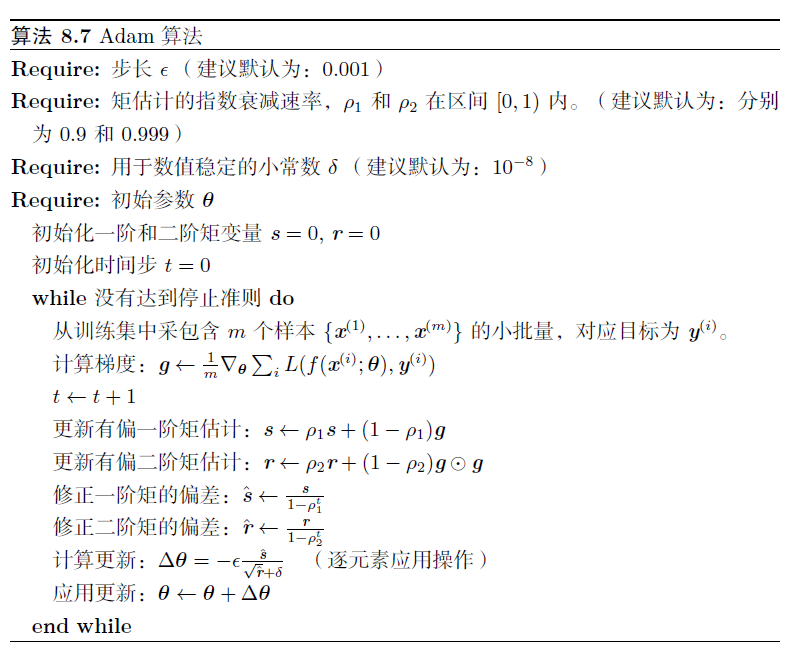
\includegraphics[width=0.8\textwidth]{adam.png}
 
    \label{fig:adm}
    \end{figure}

\subsection{建模}

\parinterval 在给定源语言句子$\mathbf{x}$的情况下, 找出翻译概率最大的目标语译文$\hat{\mathbf{y}}$:
\begin{eqnarray}
\hat{\mathbf{y}} = \argmax_{\mathbf{y}} \textrm{P} (\mathbf{y} | \mathbf{x})
\end{eqnarray}

\noindent 这里, 用$\mathbf{x}=\{ x_1, x_2, ...,  x_m \}$表示输入的源语言单词序列, $\mathbf{y}=\{ y_1, y_2, ...,  y_n \}$ 表示生成的目标语单词序列。由于神经机器自左向右逐词翻译, 并且考虑之前的结果, 因此对$\textrm{P} (\mathbf{y} | \mathbf{x})$的求解可以转换为:
\begin{eqnarray}
\textrm{P} (\mathbf{y} | \mathbf{x}) = \prod_{j=1}^{n} \textrm{P} ( y_j | \mathbf{y}_{<j },  \mathbf{x}  )
\end{eqnarray}
$ \mathbf{y}_{<j }$表示目标语第$j$个位置之前已经生成的译文单词序列。

\parinterval 求解$\textrm{P}(y_j | \mathbf{y}_{<j}, \mathbf{x})$有三个关键问题(图\ref{fig:probquestion}):

\begin{itemize}
\item	{\small\sffamily\bfseries{词嵌入}}(Word Embedding):$\mathbf{x}$和$\mathbf{y}_{<j }$的分布式表示。将源语言单词转化为实数向量。可以把这个过程记为$\textrm{e}_x (\cdot)$。类似的, $\mathbf{y}_{<j }$记为$\textrm{e}_y (\cdot)$。
\item	在词嵌入的基础上获取整个序列的表示, 即句子的{\small\sffamily\bfseries{表示学习}}(Representation Learning)。如图\ref{fig:probquestion}中, 编码器最后一个循环单元的输出$\mathbf{h}_m$被看作是一种包含了源语句子信息的表示结果, 记为$\mathbf{C}$。
\item	得到每个目标语单词的概率, 即译文单词的{\small\sffamily\bfseries{生成}}Generation)。可以用一个Softmax输出层来获取当前时刻所有单词的分布.令目标语序列$j$时刻的循环神经网络的输出向量(或状态)为$\mathbf{s}_j$。$ y_j$的生成只依赖前一个状态$\mathbf{s}_{j-1}$和当前时刻的输入。同时考虑源语言信息$\mathbf{C}$, $\textrm{P}(y_j  | \mathbf{y}_{<j}, \mathbf{x})$可以被重新定义为:
\begin{eqnarray}
\textrm{P} (y_j | \mathbf{y}_{<j}, \mathbf{x}) \equiv \textrm{P} ( {y_j | \mathbf{s}_{j-1} , y_{j-1}, \mathbf{C}} )
\end{eqnarray}
可以进一步简化为, 
\begin{eqnarray}
\textrm{P} (y_j | \mathbf{y}_{<j}, \mathbf{x}) \equiv
 \left \{ \begin{array}{ll}
\textrm{P} (y_j |\mathbf{C} , y_{j-1}) &j=1 \\
\textrm{P} (y_j|\mathbf{s}_{j-1}, y_{j-1})  \quad &j>1
\end{array} \right . 
\end{eqnarray}
\end{itemize}

\begin{figure}[htp]
    \centering
     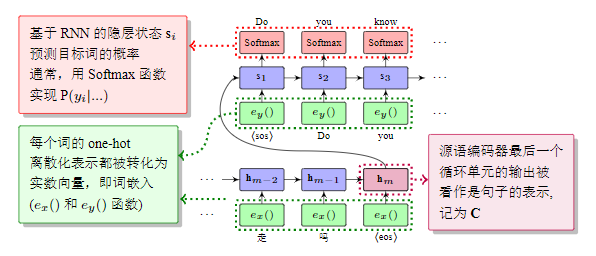
\includegraphics[width=0.8\textwidth]{RNNprobquestion.png}
    \caption{求解$\textrm{P} (y_j | \mathbf{y}_{<j}, \mathbf{x})$的三个基本问题}
    \label{fig:probquestion}
    \end{figure}

    \parinterval 那么怎么在神经机器翻译系统中获得单词的词嵌入表示呢?这里引入一个词嵌入层对输入的单词进行词嵌入表示, 即图\ref{fig:6-12}中的绿色方框部分。假设输入的单词$y_j$已经被表示为One-hot形式(行向量)。词嵌入层的工作就是把One-hot向量右乘一个实数矩阵$\mathbf{E}$, 得到的结果(行向量)就是这个单词所对应的词嵌入结果。
    \begin{eqnarray}
    \textrm{e}_y (y_j) = y_j \mathbf{E} 
    \end{eqnarray} 

    \noindent 这里, $\mathbf{E}$也被称作词嵌入矩阵, 它可以作为模型的一部分参数共同参与机器翻译系统的训练, 也可以由外部其他模块训练得到(如预训练模型)。$\mathbf{E}$的大小为$|V| \times d$, 这里$|V|$表示词表$V$的大小, $d$表示循环神经网络输入和输出向量的维度。
    

    词嵌入的作用是把离散化的单词表示转换为连续空间上的分布式表示
    \begin{enumerate}
        \item   把输入的词转换成唯一对应的词表大小的0-1向量
        \item 根据0-1向量, 从词嵌入矩阵中取出对应的词嵌入$e(\cdot)$
        \item 取出的词嵌入$e(\cdot)$作为循环神经网络的输入
    \end{enumerate} 
  
    
    
\begin{figure}[htp]
    \centering
    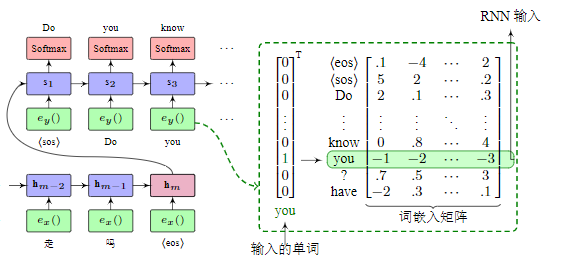
\includegraphics[width=0.8\textwidth]{NMLEmbed.png}
    \caption{词嵌入的生成过程}
 
    \end{figure}

输出层需要得到每个目标语单词的生成概率, 进而选取概率最高的词作为输出。但RNN中的隐藏层并不会输出单词概率, 而是输出s, 其每一行对应一个单词表示.
s经过权重矩阵W变成$\hat{s}$, 其隐藏层维度变换成词表的大小
$\hat{s}$经过Softmax变换得到不同词作为输出的概率, 即单词i的概率
$$p_i= Softmax(i) = \frac{{e^{\hat{s}_i}}}{{\sum_j e^{\hat{s}_j}}}$$
 


    \begin{figure}[htp]
        \centering
        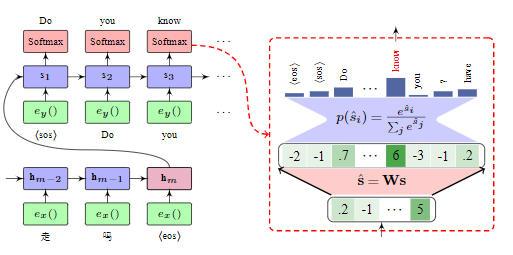
\includegraphics[width=0.8\textwidth]{outputpredict.png}
        \caption{输出层的预测过程} 
        \end{figure}

\subsubsection{RNN训练}
训练RNN我们通常会使用Adam或者SGD两种优化器, 它们各有优劣。Adam 通用, 性能不是最好, SGD  一个任务一个配置, 效果更好。
因此需要快速得到模型看一下初步效果, 选择Adam。
若是需要在一个任务上得到最优的结果, 选择SGD。
需要注意的是, 训练RNN的时候, 我们通常会遇到梯度爆炸的问题, 也就是梯度突然变得很大, 这种情况下需要使用梯度裁剪来防止梯度超过阈值。

\section{图像处理实践---ALexNet网络}
%AlexNet:ImageNet Classification with Deep Convolutional Neural Networks
 
\subsection{架构}
\subsubsection{ReLu}
对于神经元输出f建模关于输入x的函数的标准⽅法是sigmoid型函数$f(x)=\tanh(x)$或$f(x)=(1+e^{-x})$.考虑到梯度下降的训练时间, 这些饱和的非线性函数比非饱和非线性$f(x)=\max(0, x)$更慢.\textbf{采用ReLU的深度卷积神经网络训练时间比等价的tanh单元要快几倍}.

\subsubsection{局部响应归一化}

局部响应归一化(Local Response Normalization, LRN)有助于泛化.LRN的思想来源于神经生物学“侧抑制”的概念, 指的是被激活的神经元抑制周围的神经元。
定义$a_{x, y}^i$为使用核i在位置 $(x, y)$计算得到的神经元的激活值, 并应用ReLU, 响应归一化的活跃值$b_{x, y}^i $. 形如
$$b_{x, y}^i = a_{x, y}^i/(k + \alpha\sum_{j = max(0,  i-n/2)}^{min(N-1,  i + n/2)}(a_{x, y}^j))^\beta$$
其中求和在相同的空间位置遍历nnn像素邻近的核映射, NNN是该层的总核数.核映射的顺序是任意且在训练之前确定的, 该种响应归一化执行了单侧抑制, 其由真实神经元发现的该类启发, 产生了与不同核计算的神经元输出的大的激活值的对抗. 
\subsubsection{重叠池化}
池化层可以认为相距s像素的池化单元栅格, 并提取局部池化单元中中心的$z \times z$ 尺寸邻域.当$s=z$ 时, 便得到了CNN的传统局部池化;当$s<z$ 时, 便得到了重叠池化. 

\subsubsection{降低过拟合}
\paragraph{数据增强}
图像变换和水平翻转
改变训练图像的RGB通道的强度
\begin{enumerate}
    \item 随机剪切 $256 \times 256 \times 3  \to 224 \times 224 \times 3$ 
    \item 旋转处理 位置变换
    \item $224 \times 224 \times 3\to 227 \times 227 \times 3$  实际输入网络
\end{enumerate}

\subsubsection{逐层归一化(Layer-wise Normalization)}
逐层归一化是将传统机器学习中的数据归一化方法应用到深度神经网络中, 对神经网络中隐藏层的输入进行归一化, 从而使得网络更容易训练.
逐层归一化可以有效提高训练效率的原因有以下几个方面:
(1) 更好的尺度不变性.当使用随机梯度下降来训练网络时, 每次参数更新都会导致该神经层的输入分布发生改变.越高的层, 其输入分布会改变得越明显, .从机器学习角度来看, 如果一个神经层的输入分布发生了改变, 那么其参数需要重新学习, 这种现象叫作内部协变量偏移(Internal Covariate Shift). 
为了缓解这个问题, 我们可以对每一个神经层的输入进行归一化操作, 使其分布保持she稳定

(2) 更平滑的优化地形:逐层归一化一方面可以使得大部分神经层的输入
处于不饱和区域, 
\subsubsection{Dropout}
随即将一定比例的神经元置为0
对于一个有N个节点的神经网络, 有了dropout后, 就可以看做是2n个模型的集合了
相当于机器学习中的模型融合ensemble


(1)取平均的作用: 标准的模型即没有dropout, 我们用相同的训练数据去训练5个不同的神经网络, 一般会得到5个不同的结果, 此时我们可以采用 “5个结果取均值”或者“多数取胜的投票策略”去决定最终结果.例如3个网络判断结果为数字9, 那么很有可能真正的结果就是数字9, 其它两个网络给出了错误结果.这种“综合起来取平均”的策略通常可以有效防止过拟合问题.因为不同的网络可能产生不同的过拟合, 取平均则有可能让一些“相反的”拟合互相抵消.dropout掉不同的隐藏神经元就类似在训练不同的网络, 随机删掉一半隐藏神经元导致网络结构已经不同, 整个dropout过程就相当于对很多个不同的神经网络取平均.而不同的网络产生不同的过拟合, 一些互为“反向”的拟合相互抵消就可以达到整体上减少过拟合.

(2)减少神经元之间复杂的共适应关系:为dropout程序导致两个神经元不一定每次都在一个dropout网络中出现。这样权值的更新不再依赖于有固定关系的隐含节点的共同作用, 阻止了某些特征仅仅在其它特定特征下才有效果的情况。迫使网络去学习更加鲁棒的特征, 这些特征在其它的神经元的随机子集中也存在。换句话说假如我们的神经网络是在做出某种预测, 它不应该对一些特定的线索片段太过敏感, 即使丢失特定的线索, 它也应该可以从众多其它线索中学习一些共同的特征。从这个角度看dropout就有点像L1, L2正则, 减少权重使得网络对丢失特定神经元连接的鲁棒性提高。

(3)Dropout类似于性别在生物进化中的角色:物种为了生存往往会倾向于适应这种环境, 环境突变则会导致物种难以做出及时反应, 性别的出现可以繁衍出适应新环境的变种, 有效的阻止过拟合, 即避免环境改变时物种可能面临的灭绝。 

\textbf{$keep_prob$的选择}
对于不同的层, 应该设置不同的$keep_prob$, 那些神经元数量较少的层, $keep_prob$可以设置为1, 这样会保留该层所有神经元, 而那些神经元比较多的层, 可以将$keep_prob$设置为较小的值。
dropout正则化广泛运用于计算机视觉领域, 因为计算机视觉领域输入的特征一般特别多, 而且用于训练的数据较少。需要注意的是, dropout是一种正则化的方法, 在实践过程中, 除非算法出现过拟合, 否则我们不使用dropout正则化。

dropout缺点:代价函数不再被明确定义, 每次迭代, 都会随机移除一些节点, 因此无法确保成本函数单调递减。所以在使用 dropout 时, 先将$keep_prob$全部设置为 1后运行代码, 确保$J(w, b)$函数单调递减, 再打开 dropout。


\begin{figure}[!ht]
\center
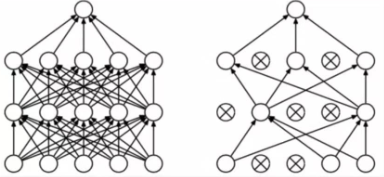
\includegraphics[width=0.8\textwidth]{dropout.png}
\end{figure}

\begin{python}
def dropout(X,  drop_prob):
    assert 0 <= drop_prob <= 1
    keep_prob = 1 - drop_prob
    if keep_prob == 0:
        return X.zeros_like()
    mask = nd.random.uniform(0,  1,  X.shape) < keep_prob
    return mask * X / keep_prob
\end{python}


\subsection{实现}

网络设计
\begin{python}
 
net = nn.Sequential()
net.add(nn.Conv2D(96,  kernel_size=11,  strides=4,  activation='relu'), 
        nn.MaxPool2D(pool_size=3,  strides=2), 
        nn.Conv2D(256,  kernel_size=5,  padding=2,  activation='relu'), 
        nn.MaxPool2D(pool_size=3,  strides=2), 
        nn.Conv2D(384,  kernel_size=3,  padding=1,  activation='relu'), 
        nn.Conv2D(384,  kernel_size=3,  padding=1,  activation='relu'), 
        nn.Conv2D(256,  kernel_size=3,  padding=1,  activation='relu'), 
        nn.MaxPool2D(pool_size=3,  strides=2), 
        nn.Dense(4096,  activation="relu"),  nn.Dropout(0.5), 
        nn.Dense(4096,  activation="relu"),  nn.Dropout(0.5), 
        nn.Dense(10))
\end{python}


如图\ref{AlexOutput1}, 学习率0.01, 迭代5次
\begin{figure}[!htb]
    \center
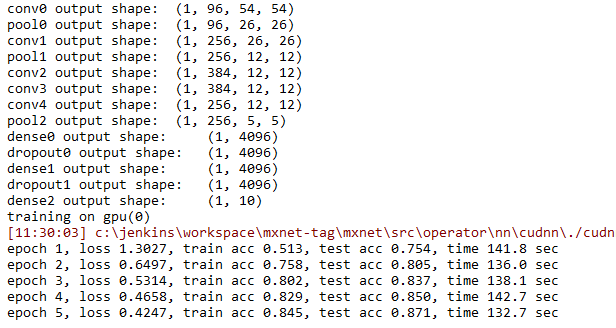
\includegraphics[width=0.8\textwidth]{alex_output.png}
\caption{AlexNet程序输出}
\label{AlexOutput1}

\end{figure}
 

如图\ref{AlexOutput2}, 学习率0.01, 训练集准确率大于92\% 终止, 共迭代27次
\begin{figure}[!ht]
    \center
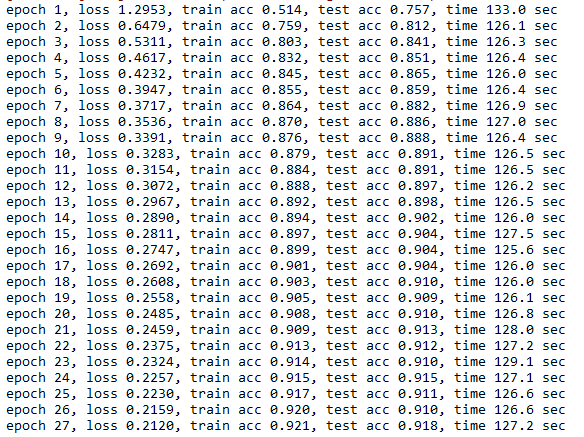
\includegraphics[width=0.8\textwidth]{alex_output3.png}
\caption{AlexNet程序输出2}
\label{AlexOutput2}

\end{figure}

如图\ref{AlexOutput3}, 利用余弦函数的单调性来完成学习率的调整, 初始学习率0.1, 最终学习率0.01, 准确率大于92\% 终止, 共迭代8次完成任务
\begin{figure}[!ht]
    \center
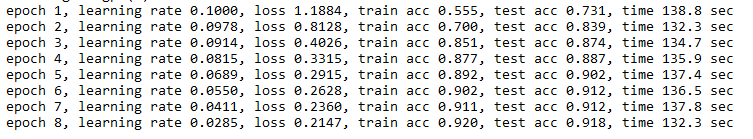
\includegraphics[width=0.8\textwidth]{alex_output4.png}
\caption{AlexNet程序输出3}
\label{AlexOutput3}

\end{figure}

\subsubsection{学习率的选择}

学习率越大, 输出误差对参数的影响就越大, 参数更新的就越快, 但同时受到异常数据的影响也就越大, 很容易发散。

如图\ref{lrselect}, 可以以非常低的学习率开始训练模型, 在每一次迭代过程中逐渐提高学习率(线性提高或指数提高, 估计出最佳学习率。 

\begin{figure}[!ht]
    \center
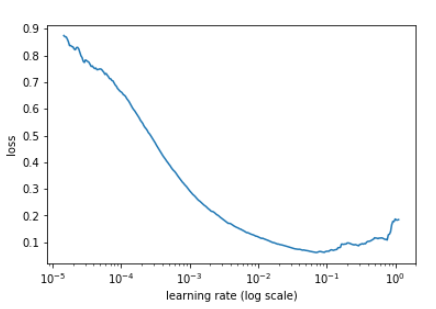
\includegraphics[width=0.4\textwidth]{lrselect.png}
\caption{随着迭代次数学习率的变化}
\label{lrselect}

\end{figure}


如图\ref{cyclelr}, 如果卡在鞍点上, 提高学习速率可以更快地穿越\textbf{鞍点}。可以使用周期学习率.
\begin{figure}[!ht]
    \center
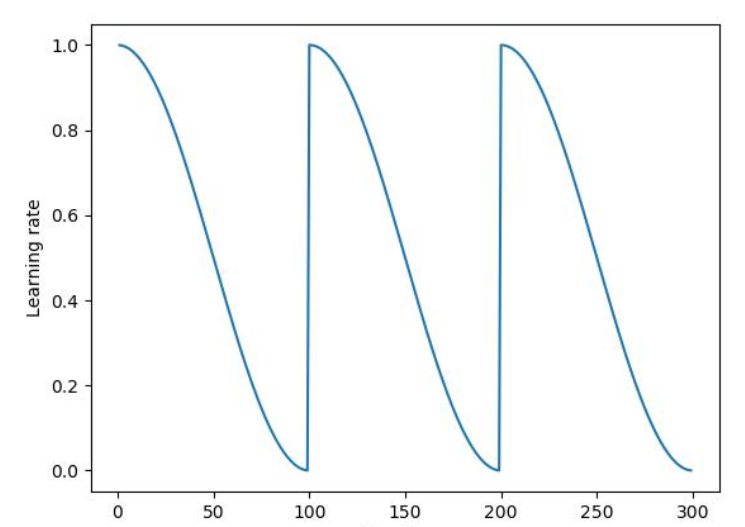
\includegraphics[width=0.4\textwidth]{cyclelr.png}
\caption{周期学习率}
\label{cyclelr}

\end{figure}


\section{联邦学习实践--FATE}
本实验使用两台虚拟机搭建联邦学习架构KubeFATE。

FATE架构如\ref{fate_architecture}所示。
\subsection{FATE架构及安装}
\begin{figure}[htb]
    \center
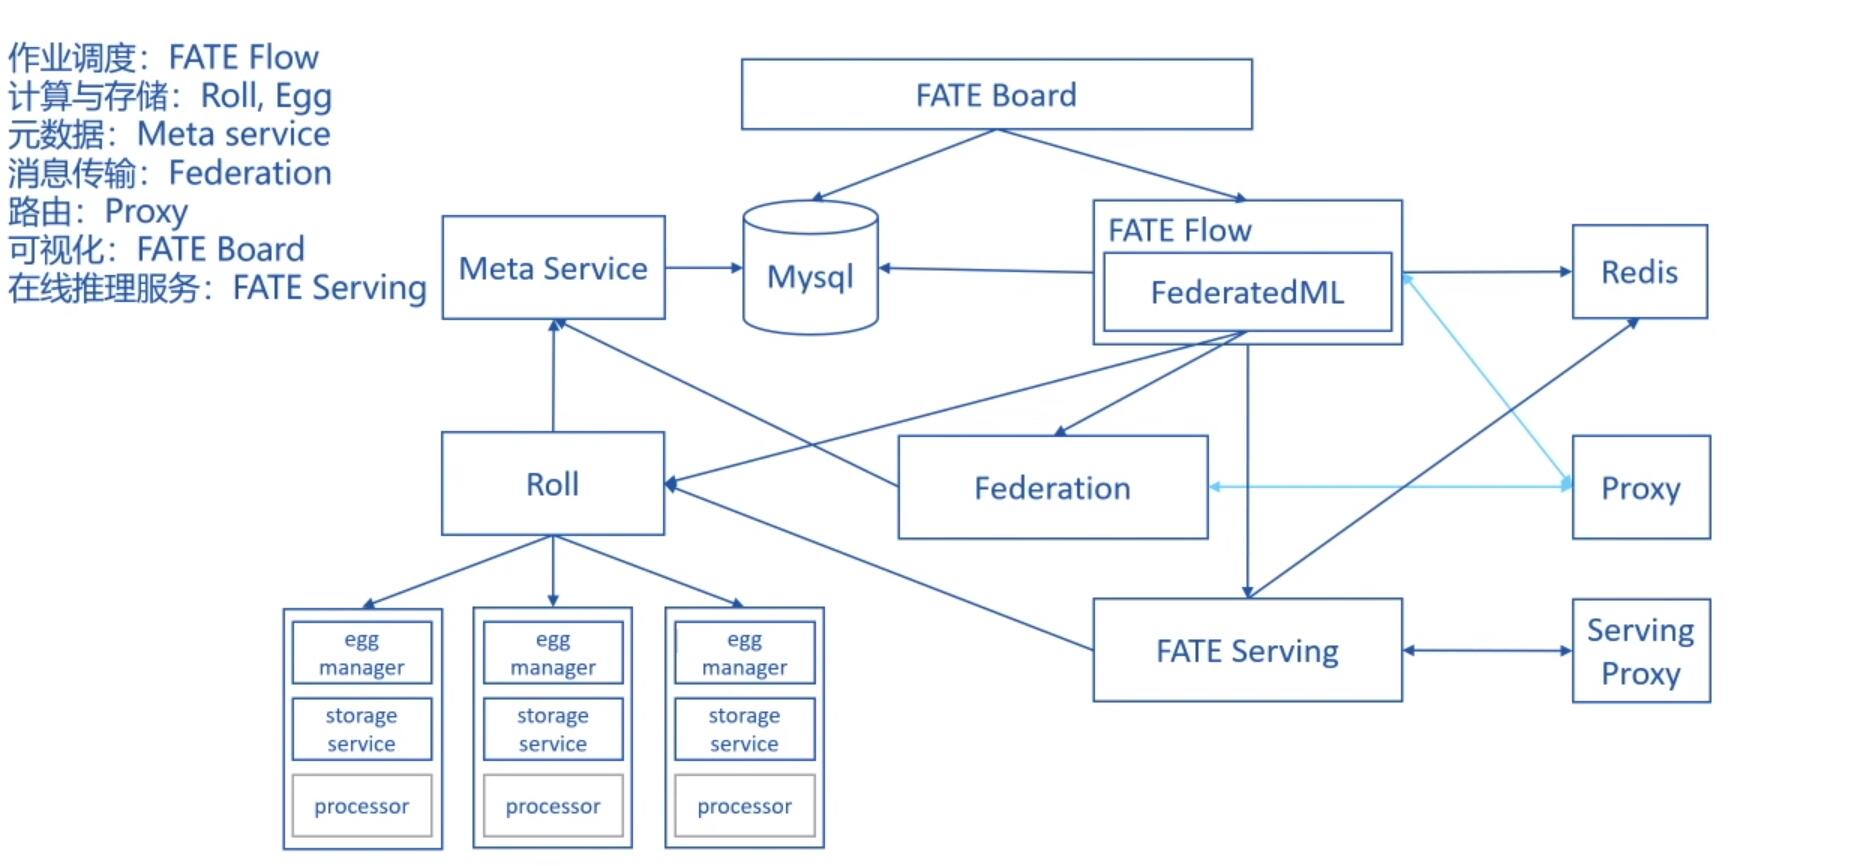
\includegraphics[width=0.8\textwidth]{fate1.jpg}
\caption{联邦学习架构}
\label{fate_architecture}
\end{figure}

准备工作
\begin{enumerate}
    \item 两个主机(物理机或者虚拟机, 都是Ubuntu系统);
    \item 所有主机安装Docker版本: 18+;
    \item 所有主机安装Docker-Compose 版本: 1.24+;
    \item 主机相互之间可以网络互通;
    \item ssh免密登录
\end{enumerate}
部署成功后使用 docker ps 命令显示如下组件, 分别对应于架构各部分。
\begin{figure}[!ht]
    \center
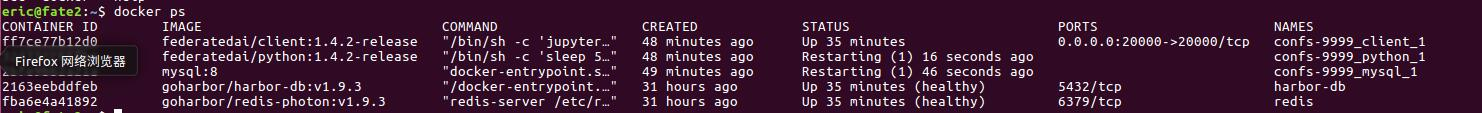
\includegraphics[width=0.8\textwidth]{fate_success.jpg}
\caption{FATE运行时各组件}
\end{figure}

\subsection{实验-利用MINST数据集进行联邦学习训练-待做}

\paragraph{初步计划}

将MINST数据集的6万调数据分为两个3万的数据集,在两台机器分别训练后再提交合并。
 
\section{个人思考}
联邦平均算法是否存在用户权重不同的情况。

联邦学习和分布式机器学习的关系。


\subsection{并行模型}

数据并行(data parallelism):不同的机器有同一个模型的多个副本, 每个机器分配到不同的数据, 然后将所有机器的计算结果按照某种方式合并。
数据并行化式的分布式训练在每个工作节点上都存储一个模型的备份, 在各台机器上处理数据集的不同部分。数据并行化式训练方法需要组合各个工作节点的结果, 并且在节点之间同步模型参数。
模型并行(model parallelism):分布式系统中的不同机器(GPU/CPU等)负责网络模型的不同部分 —— 例如, 神经网络模型的不同网络层被分配到不同的机器, 或者同一层内部的不同参数被分配到不同机器;
\begin{figure}[!ht]
    \center
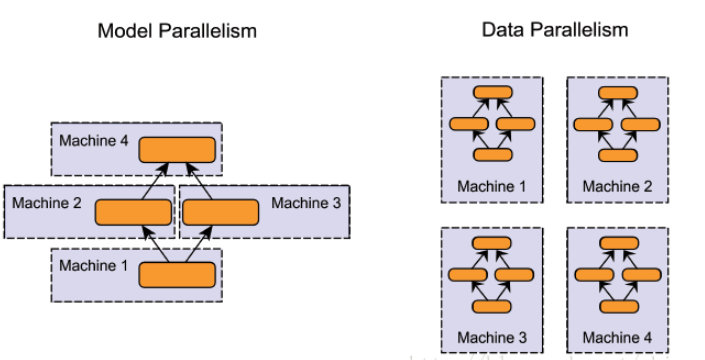
\includegraphics[width=0.4\textwidth]{paralle.png}
\caption{并行模型}
\label{parallelism}
\end{figure}


\subsubsection{AlexNet模型并行}
AleaNe的训练需要由两个GPU卡井行完成。在AexNet中, 卷积核被划分为两组, 分别在两块GPU上做模型并行训练。不过, AlexNet对模型进行了一定的修改。依照常规的模型并行逻辑, 每层神经网络的计算过程中都会发生通信, 然而在AlexNet中, 第一个卷积层到第二个卷积层、第三个卷积层到第四个卷积层以及第四个卷积层到第五个卷积层的两路计算之间没有依赖, 因而无须交互和通信。这样做主要是为了减少通信的数据量, 提高并行的效率。
基于模型井行的算法从直观上可以理解成把多个工作节点虚拟化为一个巨大的计算节点。在计算过程中模型划分越多, 交互和通信也将越多, 并且任何一个工作节点出现问题整个计算都会受到影响, 因此鲁棒性欠佳。AlexNet 在提高效率方面进行了有益的尝试, 通过在模型设计中放弃些交互, 换来整体效率的提升。

模型并行与联邦学习中模型的合并

 


\subsection*{一些词汇}
\subsubsection*{ Cross-Silo} 
silo 的本意是地窖、竖井, cross-silo 里的silo是指“信息孤井”, 信息孤岛.所谓信息孤井就是指, 一个企业中各个部门的信息系统相互独立, 各自为战, 没有联系, 就像一口口孤井.这样的结果显然是效率降低, 信息重复度高, 易冲突出错.因此出现 cross-silo 的概念, 就是打通这些孤井, 让它们连成一体, 这样将提高信息一致性、提高效率, 而且有利于准确分析.
所以 cross-silo 可以翻成 孤井互连, 或者孤井互通等. 

% \subsubsection*{vanilla拆分学习}
% vanilla除了香草的意思以外还有原始的, 普通的意思, 比如vanilla neural network, 指普通神经网络  .
% 有什么想法都可以先记下来, 暂时没有进展不要紧.

\subsection{待解决}
算法挑战
%%=====参考文献===============
%% 这里做好bib文件的维护, 对于文献的引用名按如下格式命名:期刊简称-第一作者姓-第二作者姓-etc年份(超过两个作者, 只列前两个作者, 其余的用etc代替)
PySyft中的联邦学习 

\bibliography{references}

%%Xing,  H.,  Simeone,  O.,  & Bi,  S. (2020). Decentralized Federated Learning via SGD over Wireless D2D Networks. arXiv preprint arXiv:2002.12507.


\end{document}
